\documentclass[12pt,letterpaper]{article}
\usepackage{amsmath,amssymb}
\usepackage{graphicx}
\usepackage{bm}
\usepackage{physics}
\usepackage{authblk}
\usepackage{setspace}
\usepackage{geometry}
\usepackage[labelfont=bf]{caption}
\usepackage[colorlinks=true,linkcolor=blue,citecolor=blue,urlcolor=blue]{hyperref}
\usepackage{tabularx}
\usepackage{ragged2e}
\usepackage{booktabs}

\geometry{
  letterpaper,
  top=2.5cm,
  bottom=2.5cm,
  left=2.5cm,
  right=2.5cm
}

\usepackage{tikz}
\usetikzlibrary{decorations.pathmorphing,arrows.meta, calc, 3d, shadings, positioning}

\onehalfspacing

% ========================================
% Document Begin
% ========================================

\begin{document}

% ========================================
% Title and Front Matter
% ========================================

\title{Detailed Exposition of the 0-Sphere Model Framework\\
for Gravitational-Like Phenomena\\
\normalsize Supplementary Note to ``Geometrical Confinement of Energy in the 0-Sphere Model''}

\author{Satoshi Hanamura
\thanks{Email: hana.tensor@gmail.com}}

\date{February 7, 2026}

\maketitle

\tableofcontents

% ========================================
% Research Summary
% ========================================

\begin{center}
\textbf{Research Summary}
\end{center}

\justifying

This supplementary document provides a comprehensive exposition of the theoretical framework presented in the main manuscript, ``Geometrical Confinement of Energy in the 0-Sphere Model: A Topological Mechanism Underlying Rest Mass, Zitterbewegung, and Gravitational-Like Phenomena~\cite{Hanamura2026geometrical}.''

The primary purpose of this supplement is to make the conceptual structure, physical motivation, and broader implications of the 0-Sphere model accessible to a wider audience, including researchers in adjacent fields, graduate students, and readers seeking a deeper understanding of the paradigm shift proposed in the main text.

The main manuscript, written in the concise technical style appropriate for specialist audiences, necessarily builds upon the core principles of quantum mechanics, general relativity, and thermodynamics. In contrast, the present supplementary exposition adopts a more pedagogical approach, bridging the gap between traditional perspectives and the novel conceptual framework of the 0-Sphere model. By providing a more intuitive walkthrough of these foundational elements, this supplement aims to facilitate a smoother transition into the model's unique shift in perspective, ensuring that its core insights are accessible to a broader range of researchers. To this end, it elaborates on:

\begin{itemize}
\item \textbf{Why this research is necessary:} The conceptual tensions in existing theoretical frameworks and the unresolved problems that motivate the development of the 0-Sphere model
\item \textbf{What the model proposes:} A step-by-step exposition of the core mechanisms, from individual electrons to macroscopic, gravity-like phenomena
\item \textbf{How it differs from conventional approaches:} The foundational shift from a field-theoretic description to a line-integral-based ontology
\item \textbf{What remains to be solved:} Open questions, theoretical limitations, and directions for future investigation
\item \textbf{What it means for physics:} Philosophical and practical implications for quantum gravity, experimental tests, and the interpretation of spacetime
\end{itemize}

This document is structured to guide readers through progressively deeper levels of understanding, beginning with foundational questions and advancing toward the quantitative predictions and unresolved challenges discussed in the main manuscript. In doing so, it is intended not only to function as a companion text that enhances comprehension of the technical content while maintaining scientific rigor, but also to consolidate and contextualize elements developed across the author's prior studies, thereby providing a coherent reference framework that facilitates appropriate citation and reuse.

% ========================================
% Section 1: Background and Motivations
% ========================================

\section{Background and Motivations}
\label{sec:background}

\justifying

% ----------------------------------------
% Subsection 1.1: The Two Pillars
% ----------------------------------------

\subsection{The Two Pillars of Modern Physics}
\label{subsec:two_pillars}

Contemporary physics is founded on two remarkably successful theoretical frameworks. General relativity (GR) describes gravitation as the curvature of spacetime, accurately accounting for phenomena ranging from planetary motion to black hole dynamics and cosmological expansion. Quantum field theory (QFT), by contrast, unifies three of the four known fundamental interactions—electromagnetic, weak, and strong—within the Standard Model of particle physics, achieving a level of predictive precision unparalleled in the physical sciences.

Despite their respective successes, these two pillars remain fundamentally incompatible. General relativity is a classical theory formulated on a smooth spacetime continuum, whereas quantum field theory is intrinsically probabilistic and relies on field quantization. Efforts to reconcile these frameworks within a consistent theory of quantum gravity have, despite decades of sustained work, encountered deep mathematical and conceptual difficulties. These challenges motivate continued exploration of alternative formulations that revisit the assumptions underlying both field-based descriptions and continuum spacetime.

% ----------------------------------------
% Subsection 1.2: Pointwise Field Values
% ----------------------------------------

\subsection{The Implicit Assumption: Pointwise Field Values}
\label{subsec:pointwise_fields}

Both GR and QFT share a common conceptual foundation: \textbf{the assumption that physical quantities are defined at every point in spacetime}. In GR, the metric tensor $g_{\mu\nu}(x)$ assigns geometric properties to each point. In QFT, field operators $\phi(x)$ are defined at each spacetime coordinate. Forces arise as gradients of these fields, and dynamics are governed by differential equations relating neighboring points.

This picture, while mathematically elegant and empirically successful, carries implicit ontological commitments. What is a ``point'' in spacetime? Is it an observable entity, or merely a calculational convenience? The unobservable ``coordinate mesh'' permeating all of space—dense, continuous, and infinitely divisible—has never been directly verified.

Moreover, the very notion of a point becomes problematic at the Planck scale ($\sim 10^{-35}$ m), where quantum fluctuations of spacetime itself are expected to become significant. The smooth continuum picture may be an emergent, effective description valid only at macroscopic scales, masking a fundamentally different microscopic structure.

% ----------------------------------------
% Subsection 1.3: The Graviton Problem
% ----------------------------------------

\subsection{The Graviton Problem}
\label{subsec:graviton}

Within the framework of quantum field theory, fundamental interactions are described as being mediated by gauge bosons: photons for electromagnetism, $W$ and $Z$ bosons for the weak interaction, and gluons for the strong interaction. By analogy, gravity is commonly hypothesized to be mediated by a corresponding quantum excitation, referred to as the \textbf{graviton}.

To date, however, no direct experimental evidence for gravitons has been obtained. More significantly, attempts to formulate a consistent quantum field theory of gravity face persistent technical obstacles. Perturbative treatments of graviton interactions are non-renormalizable, in the sense that quantum corrections generate divergences that cannot be absorbed into a finite set of physical parameters within the standard framework of field theory. This behavior contrasts sharply with the renormalizable structure of the gauge theories underlying the Standard Model.

As a consequence, general relativity is widely regarded as an effective description, expected to lose validity near the Planck scale. Various candidate frameworks—such as string theory, loop-based approaches, and other non-perturbative constructions—have been proposed as possible ultraviolet completions, but none has yet achieved empirical confirmation.

This situation motivates a more basic reconsideration: \textbf{is the graviton a necessary constituent of physical reality, or does its apparent necessity arise from extending field-theoretic concepts into a regime where the underlying interaction may not be fundamentally field-like at all?}

% ----------------------------------------
% Subsection 1.4: Origin of Inertial Mass
% ----------------------------------------

\subsection{The Origin of Inertial Mass}
\label{subsec:inertial_mass}

Another fundamental question concerns the origin of inertial mass: why do physical systems resist acceleration? The Higgs mechanism provides a partial answer by explaining how elementary particles acquire rest mass through interactions with the Higgs field. However, this contribution accounts for only a small fraction—of order one percent—of the mass budget of ordinary matter. The dominant contribution arises from the binding energy of quarks and gluons within nucleons, as described by quantum chromodynamics (QCD).

Even so, this explanation remains incomplete at a conceptual level. The Higgs mechanism and QCD successfully account for the \textit{magnitude} of mass, but they do not fully address what inertia \textit{is}. Why does a system endowed with internal energy require a force to change its state of motion? What microscopic process underlies this resistance to acceleration?

If inertial mass ultimately originates from internal energy—whether associated with the Higgs field, QCD binding, or other internal degrees of freedom—then a deeper connection between internal dynamics and gravitational behavior may exist. Exploring this possibility motivates frameworks in which mass, inertia, and gravity are not treated as independent primitives, but as emergent consequences of underlying dynamical structure.

% ----------------------------------------
% Subsection 1.5: Motivation for New Approach
% ----------------------------------------

\subsection{Motivation for a New Approach}
\label{subsec:new_approach}

These conceptual and technical challenges motivate consideration of alternative formulations. Rather than assuming continuous fields as fundamental and subsequently seeking to quantize them, one may instead ask whether \textbf{discrete, history-dependent structures} could provide a more suitable starting point.

The 0-Sphere model explores such a possibility by treating \textbf{line integrals of phase histories} as the primary physical observables, replacing pointwise field values. This shift is not merely a change of mathematical representation; it reflects an attempt to reframe how interactions, inertial mass, and gravitational-like phenomena might arise from underlying dynamical processes.

% ========================================
% Section 2: Core Concept
% ========================================

\section{Core Concept: From Fields to Line Integrals}
\label{sec:core_concept}

\justifying

% ----------------------------------------
% Subsection 2.1: Ontological Shift
% ----------------------------------------

\subsection{The Ontological Shift}
\label{subsec:ontological_shift}

At the core of the 0-Sphere model lies a shift in ontology, understood here as a change in what is taken to be the primary carrier of physical information.

\textbf{Conventional field-based descriptions:}
\begin{itemize}
\item Spacetime is treated as a continuous manifold
\item Physical fields $\phi(x)$ are defined at each spacetime point $x$
\item Forces are typically associated with local gradients, $F \propto -\nabla \phi$
\item Interactions are assumed to be local in spacetime
\end{itemize}

\textbf{Line-integral-based description explored in the 0-Sphere model:}
\begin{itemize}
\item Physical observables are defined as line integrals along trajectories
\item Phase accumulation, $\Theta = \int_\gamma d\theta$, plays a central role
\item Interactions depend on cumulative phase histories rather than instantaneous field values
\item Spacetime relations arise from the resulting relational structure
\end{itemize}

This represents more than a change of mathematical representation. Line integrals are intrinsically path-dependent, encoding the full interaction history of a system. As a consequence, two systems that are identical at an instantaneous level but differ in their past trajectories may exhibit different accumulated phases, leading to distinct subsequent dynamics.

% ----------------------------------------
% Subsection 2.2: Empirical Precedents
% ----------------------------------------

\subsection{Empirical Precedents: Aharonov--Bohm, Berry Phase, Wilson Loops}
\label{subsec:empirical_precedents}

A line-integral-based description of physical observables is not without empirical precedent. Several well-established phenomena in quantum physics already assign a fundamental role to phase accumulation along closed or extended paths.

\textbf{Aharonov--Bohm effect:} An electron encircling a solenoid acquires a measurable phase shift even when the magnetic field vanishes along its trajectory. The phase depends on the line integral of the vector potential,
\begin{equation}
\Delta \theta = \frac{e}{\hbar} \oint \bm{A} \cdot d\bm{\ell}.
\end{equation}
This effect illustrates that gauge potentials can have observable consequences through path-dependent phase accumulation, independent of local field strengths.

\textbf{Berry phase:} When a quantum system undergoes adiabatic evolution along a closed loop in parameter space, it acquires a geometric phase,
\begin{equation}
\gamma = \oint \bm{A}_{\mathrm{Berry}} \cdot d\bm{R},
\end{equation}
which depends only on the trajectory in parameter space and has experimentally verified interference effects.

\textbf{Wilson loops:} In gauge theories, the holonomy around a closed contour,
\begin{equation}
W[\mathcal{C}] = \mathrm{Tr}\, \mathcal{P} \exp\!\left( i \oint_{\mathcal{C}} A_\mu \, dx^\mu \right),
\end{equation}
defines a gauge-invariant observable that characterizes the global structure of the gauge field configuration.

The 0-Sphere framework can be viewed as extending this line of thought by exploring whether such path-dependent quantities may serve not merely as auxiliary constructs, but as the primary carriers of physical information.

% ----------------------------------------
% Subsection 2.3: Open Paths vs Closed Loops
% ----------------------------------------

\subsection{From Closed Loops to Open Paths: A Fundamental Distinction}
\label{subsec:open_paths}

The examples discussed above—Aharonov--Bohm effect, Berry phase, and Wilson loops—share a common mathematical structure: they are defined as line integrals around \textbf{closed contours},
\begin{equation}
\Theta_{\mathrm{closed}} = \oint_{\mathcal{C}} \mathcal{A} \cdot d\bm{\ell},
\end{equation}
where the initial and final points coincide. Such closed-loop integrals represent \textbf{cyclic phase accumulation}, encoding gauge-invariant or geometric information that can manifest as interference effects when an observer or quantum state returns to its starting configuration.

The 0-Sphere framework, by contrast, assigns fundamental physical significance to line integrals along \textbf{open paths}:
\begin{equation}
\Theta_{\mathrm{open}} = \int_{\gamma: A \to B} d\theta,
\end{equation}
where the initial point $A$ and the final point $B$ are distinct. This is not a technical variation but reflects a shift in ontology: rather than describing cyclic interference phenomena superimposed on a fixed spacetime background, open-path line integrals represent the \textbf{actual transport of energy and phase} along physical trajectories.

Three key distinctions clarify this difference:

\textbf{1. Cyclic vs. Directional Transport}
\begin{itemize}
\item \textbf{Closed loops:} Phase accumulation returns to the initial state, manifesting as relative phase shifts in interference patterns. The system explores parameter space but does not undergo net displacement.
\item \textbf{Open paths:} Energy and phase are transported from kernel $A$ to kernel $B$ along a geodesic trajectory. This transport is directional and irreversible, reflecting thermodynamic evolution.
\end{itemize}

\textbf{2. Parameter Space vs. Real Space}
\begin{itemize}
\item \textbf{Berry phase:} The closed loop occurs in an abstract parameter space. Physical position may remain unchanged even as geometric phase accumulates.
\item \textbf{0-Sphere:} The trajectory $\gamma$ represents motion through real space, where a particle or energy quantum actually moves from one location to another along a thermally preferred path.
\end{itemize}

\textbf{3. Gauge Potentials vs. Thermal Geodesics}
\begin{itemize}
\item \textbf{Conventional line integrals:} The connection $\mathcal{A}$ (vector potential, Berry connection, gauge field) exists on a pre-defined spacetime manifold.
\item \textbf{0-Sphere:} Spacetime structure itself emerges from accumulated interaction histories. The ``connection'' is not imposed externally but arises from the phase network topology. Geodesics are determined thermodynamically rather than geometrically prescribed.
\end{itemize}

This distinction has profound implications. In conventional gauge theories, Wilson loops characterize the global structure of a gauge field defined on a fixed background. In the 0-Sphere model, open-path line integrals define the relational structure from which spacetime geometry itself emerges. The question is not ``what is the holonomy around a given contour?'' but rather ``how does accumulated phase history along interaction pathways give rise to effective spacetime relations?''

The shift from closed to open line integrals therefore marks the transition from \textbf{gauge-theoretic phase accumulation on a background} to \textbf{ontologically primary phase histories that constitute spacetime structure}.

% ----------------------------------------
% Subsection 2.4: The 0-Sphere Structure
% ----------------------------------------

\subsection{The 0-Sphere Structure}
\label{subsec:0sphere_structure}

% Two-Kernel Geometry
\subsubsection{Two-Kernel Geometry and Radiative Coupling}
\label{subsubsec:two_kernel}

The term ``0-Sphere'' refers to the zero-dimensional sphere $S^0$, representing a \textbf{configuration space of two discrete points}. This does not mean that the electron consists of two spatially separated objects connected by a ``string.'' Rather, $S^0$ characterizes the set of \textbf{possible energy localization sites} between which the electron's total energy oscillates through radiative transport.

At any given instant, characterized by the internal phase $\theta(t) = \omega t$, the electron's energy is \textbf{predominantly localized at a single kernel}. When $\theta = 0$ (or integer multiples of $2\pi$), 100\% of the energy resides at kernel $A$. When $\theta = \pi$ (or odd multiples of $\pi$), 100\% of the energy has been transported to kernel $B$. The transition between these configurations occurs through continuous radiative exchange, not through the persistence of a static two-body structure.

Importantly, the electron's energy \textit{can} occupy both kernels simultaneously during certain time phases. This is made explicit by the energy conservation identity of the 0-Sphere Model,
\begin{equation}
  E_0 = \underbrace{\cos^4\!\theta}_{E_A\;(\text{Kernel }A)} + \underbrace{\sin^4\!\theta}_{E_B\;(\text{Kernel }B)} + \underbrace{\tfrac{1}{2}\sin^2\!(2\theta)}_{E_{\mathrm{trans}}\;(\text{photon sphere})}, \qquad \theta = \frac{\omega\, t}{2}.
  \label{eq:energy_conservation}
\end{equation}
Here $E_A$ and $E_B$ denote the thermal potential energies of kernel $A$ and kernel $B$, respectively, and $E_{\mathrm{trans}}$ is the transition kinetic energy carried through the photon sphere. The right-hand side is identically unity for all $\theta$, since
\[
  \cos^4\!\theta + \sin^4\!\theta + 2\sin^2\!\theta\,\cos^2\!\theta = \bigl(\cos^2\!\theta + \sin^2\!\theta\bigr)^2 = 1,
\]
guaranteeing energy conservation at every instant.

At $\theta = 0$ and $\theta = \pi/2$, all thermal potential energy resides in a single kernel:
\begin{align}
  \theta = 0:\qquad\quad &E_0 = \underbrace{1}_{E_A} + \underbrace{0}_{E_B} + \underbrace{0}_{E_{\mathrm{trans}}} = 1, \\[6pt]
  \theta = \frac{\pi}{2}:\qquad &E_0 = \underbrace{0}_{E_A} + \underbrace{1}_{E_B} + \underbrace{0}_{E_{\mathrm{trans}}} = 1.
\end{align}
These are the \textit{one-point contact} phases in the inchworm analogy. At the intermediate phase $\theta = \pi/4$, however, both kernels are occupied equally:
\begin{equation}
  \theta = \frac{\pi}{4}:\qquad E_0 = \underbrace{\tfrac{1}{4}}_{E_A} + \underbrace{\tfrac{1}{4}}_{E_B} + \underbrace{\tfrac{1}{2}}_{E_{\mathrm{trans}}} = 1.
\end{equation}
This is the \textbf{dumbbell configuration}: kernels $A$ and $B$ share their thermal potential energy equally, and at this very phase the transition kinetic energy $E_{\mathrm{trans}}$ simultaneously reaches its maximum value $\tfrac{1}{2}$. In other words, the photon sphere is most energetically active at precisely the moment when the two kernels are symmetrically occupied. In the inchworm analogy, this corresponds to the \textit{two-point contact} state.

The characteristic separation between these localization sites is taken to be of the order of the Compton wavelength,
\begin{equation}
\lambda_C = \frac{\hbar}{m_e c} \approx 2.4 \times 10^{-12} \, \mathrm{m}.
\end{equation}
This defines the \textbf{spatial extent of the oscillatory cycle}, not a fixed distance between coexisting objects.

Crucially, this is not a ``virtual oscillation'' in the sense of unobservable quantum fluctuations. The energy transport $A \to B \to A'$ is a real, thermodynamically sustained process involving the emission, propagation, and absorption of photons. These are \textbf{real photons}, on-shell and in principle observable, satisfying the relativistic dispersion relation $E = pc$. Because photons carry zero chemical potential ($\mu = 0$), the maintenance of this radiative exchange does not require photon number conservation, only the persistence of energy flow within the photon sphere.

The two kernels, $A$ and $B$, therefore represent \textbf{phase-dependent energy configurations} rather than independent degrees of freedom. At $\theta = 0$, the system is ``at kernel $A$.'' At $\theta = \pi$, the system is ``at kernel $B$.'' The photon sphere provides arcwise connectivity between these states, enabling the definition of line integrals
\begin{equation}
\Theta = \int_{\gamma: A \to B} d\theta
\end{equation}
along the \textbf{actual trajectory of energy transport}, not a closed loop in parameter space.

% Inchworm Analogy
\subsubsection{Phase-Dependent Energy Localization: The Inchworm Analogy}
\label{subsubsec:inchworm}

To further clarify the non-static character of the 0-Sphere structure, consider the phase-dependent energy distribution governed by the energy conservation identity:
\begin{equation}
  E_0 = \underbrace{\cos^4\!\theta}_{E_A\;(\text{Kernel }A)} + \underbrace{\sin^4\!\theta}_{E_B\;(\text{Kernel }B)} + \underbrace{\tfrac{1}{2}\sin^2\!(2\theta)}_{E_{\mathrm{trans}}\;(\text{photon sphere})}, \qquad \theta = \frac{\omega\,t}{2}.
\end{equation}
Here $E_A$ and $E_B$ denote the thermal potential energies localized at kernel $A$ and kernel $B$, respectively, and $E_{\mathrm{trans}}$ is the transition kinetic energy carried through the photon sphere. The fourth-power dependence of $E_A$ and $E_B$ arises from the Stefan--Boltzmann radiation law applied to thermal emission and absorption at each kernel. The right-hand side is identically unity for all $\theta$, since
\[
  \cos^4\!\theta + \sin^4\!\theta + 2\sin^2\!\theta\,\cos^2\!\theta = \bigl(\cos^2\!\theta + \sin^2\!\theta\bigr)^2 = 1,
\]
guaranteeing energy conservation at every instant of the continuous phase evolution.

Three representative phases are particularly instructive. At $\theta = 0$ and $\theta = \pi/2$, all thermal potential energy resides in a single kernel:
\begin{align}
  \theta = 0:\qquad\quad &E_0 = \underbrace{1}_{E_A} + \underbrace{0}_{E_B} + \underbrace{0}_{E_{\mathrm{trans}}} = 1, \\[6pt]
  \theta = \frac{\pi}{2}:\qquad &E_0 = \underbrace{0}_{E_A} + \underbrace{1}_{E_B} + \underbrace{0}_{E_{\mathrm{trans}}} = 1.
\end{align}
At these phases the photon sphere carries no energy, and the system is in a state of complete localization. At the intermediate phase $\theta = \pi/4$, however, both kernels are occupied equally:
\begin{equation}
  \theta = \frac{\pi}{4}:\qquad E_0 = \underbrace{\tfrac{1}{4}}_{E_A} + \underbrace{\tfrac{1}{4}}_{E_B} + \underbrace{\tfrac{1}{2}}_{E_{\mathrm{trans}}} = 1.
\end{equation}
This is the \textbf{dumbbell configuration}: kernels $A$ and $B$ share their thermal potential energy equally, and at this very phase the transition kinetic energy $E_{\mathrm{trans}}$ simultaneously reaches its maximum value of $\tfrac{1}{2}$. The photon sphere is therefore most energetically active at precisely the moment when the two kernels are symmetrically occupied. Because the electron's thermal potential energy is converted into radiative energy during transport, the photon sphere acquires a finite spatial extent on the order of the Compton wavelength; it is not a rigid rod or string, but a spatially extended radiative medium. Kernels $A$ and $B$ alternately undergo radiation and absorption cycles \textit{inside} this photon sphere --- if one adopts a soap bubble as an analogy for the photon sphere, the entirety of this energy exchange could be a phenomenon occurring within the interior of that bubble.

This phase-dependent structure is captured by the inchworm analogy. An inchworm maintains one or two points of contact with the substrate at any given instant: during the stance phases it rests on a single anchor, and during the transfer it briefly contacts the substrate at two points simultaneously. The 0-Sphere electron behaves analogously. It alternates between single-kernel localization --- the \textit{one-point contact} state at $\theta = 0$ and $\theta = \pi/2$ --- and symmetric dual-kernel occupancy --- the \textit{two-point contact} state at $\theta = \pi/4$. The transition between these states is governed by continuous, deterministic phase evolution $\theta = \omega\,t/2$, driven by the radiation-absorption cycles within the photon sphere, rather than by discrete jumps or probabilistic collapse.

% Photon Sphere as Geodesic
\subsubsection{Photon Sphere as Geodesic Structure}
\label{subsubsec:photon_sphere}

The photon sphere introduced in the previous discussion plays a dual role in the 0-Sphere framework:

\textbf{1. Geometric Scaffold:} It provides arcwise connectivity between kernels $A$ and $B$, establishing a well-defined notion of ``path'' in the absence of a pre-existing spacetime manifold.

\textbf{2. Thermal Geodesic:} It defines the thermodynamically preferred trajectory for energy and phase transport, analogous to how timelike geodesics in general relativity represent paths of extremal proper time.

Unlike field theories, where interactions occur ``at a distance'' through the exchange of virtual quanta propagating in a background spacetime, the 0-Sphere model requires an explicit geometric pathway connecting discrete energy configurations. The photon sphere \textit{is} this pathway—a dynamically sustained radiative structure along which energy and phase information are transported.

This transport process is both \textbf{directional} and \textbf{history-dependent}. When kernel $A$ oscillates with phase $\theta_A(t) = \omega_A t$, it continuously radiates energy into the photon sphere. This energy propagates along the arc connecting $A$ to $B$, where it is subsequently absorbed, thereby influencing the phase evolution $\theta_B(t)$. The line integral
\begin{equation}
\Theta = \int_{\gamma: A \to B} d\theta
\end{equation}
accumulates the phase change along this physical trajectory $\gamma$, which is crucially \textbf{not closed}. It represents actual displacement from kernel $A$ to kernel $B$, encoding both the energetic cost of the transfer and the relational phase structure established by the interaction.

% Thermodynamic Irreversibility
\subsubsection{Open Paths and Thermodynamic Irreversibility}
\label{subsubsec:thermodynamic_irreversibility}

The open character of 0-Sphere line integrals is not incidental—it reflects the \textbf{irreversible, thermodynamically driven} nature of phase network evolution.

Consider the contrast:
\begin{itemize}
\item \textbf{Aharonov--Bohm effect:}
An electron propagates from a common source to a common detector along two distinct \emph{open} paths that pass on opposite sides of a solenoid. Along both paths the magnetic field vanishes, so no classical Lorentz force acts on the electron; however, the vector potential $\bm{A}$ is non-zero, and the quantum phase accumulated along each path differs. The resulting phase difference is given by
\[
  \Delta\phi
  = \frac{e}{\hbar}
    \left[
      \int_{\text{path 1}} \bm{A}\cdot d\bm{\ell}
      -
      \int_{\text{path 2}} \bm{A}\cdot d\bm{\ell}
    \right]
  = \frac{e}{\hbar}\oint \bm{A}\cdot d\bm{\ell}
  = \frac{e}{\hbar}\,\Phi_B,
\]
and manifests experimentally as a shift of the interference pattern at the detector. The closed-loop
integral $\oint$ here is a mathematical rewriting of the difference between two open-path integrals: the electron itself does not traverse a closed trajectory, nor does it return to its initial dynamical state. The phase shift depends solely on the magnetic flux $\Phi_B$ enclosed between the paths and is therefore topologically determined, non-dissipative, and free of thermodynamic irreversibility.

\item \textbf{0-Sphere entropic entrainment:}
A subsystem whose characteristic frequency $\nu_b$ exceeds the ambient frequency $\nu_a$ becomes phase-synchronized through dissipative coupling to its environment. Internal vibrational energy is irreversibly transferred into the radiative medium of the photon sphere, driving the subsystem toward synchronization with the surrounding
ensemble. The accumulated phase depends on the full history of the coupling; the system does not return to its initial state, and the process exhibits genuine thermodynamic irreversibility.
\end{itemize}

The thermodynamic arrow of time is therefore built into the 0-Sphere formalism. Open-path line integrals naturally encode entropy increase, energy redistribution, and the emergence of macroscopic directionality from microscopic phase dynamics.

% Emergent Spacetime
\subsubsection{From Gauge Potentials to Emergent Spacetime}
\label{subsubsec:emergent_spacetime}

In conventional gauge theories, the gauge potential $A_\mu(x)$ is defined at every spacetime point $x$ on a pre-existing manifold. Physical observables, such as Wilson loops, are then constructed as functionals of these potentials.

The 0-Sphere framework inverts this hierarchy:
\begin{enumerate}
\item \textbf{Primary:} Line integrals $\int_\gamma d\theta$ representing accumulated phase histories along interaction trajectories.
\item \textbf{Derived:} Effective spacetime relations emerge from the topology of the phase network—the web of all such interaction histories.
\item \textbf{Secondary:} Pointwise field values, if needed, can be reconstructed from gradients of accumulated phase.
\end{enumerate}

This ontological reordering has several consequences:

\textbf{(a) No Background Dependence:} Spacetime structure is not assumed but emerges from the pattern of interactions. There is no ``stage'' on which physics unfolds; the stage itself is built from physical processes.

\textbf{(b) Causal Structure from Photon Exchange:} Temporal ordering arises from the causal propagation of photons at light speed. Two events are causally connected if and only if a photon can propagate between them, that is, if the light-travel time separating them does not exceed their temporal separation. No pre-existing spacetime geometry is invoked; causal ordering is built entirely from the possibility or impossibility of photon exchange.

\textbf{(c) Metric Relations from Phase Gradients:} Effective distances can be inferred from phase synchronization scales. The time required for a photon, propagating at speed $c$, to traverse the interval between two subsystems sets a fundamental causal bound on how rapidly phase synchronization can occur. Subsystems connected by short light-travel times can establish phase correlations rapidly and are operationally ``close,'' whereas those separated by long light-travel times can synchronize only over correspondingly longer timescales and are ``distant.''

This approach resonates with relational perspectives in quantum gravity, where spacetime is not fundamental but emerges from the relational structure of events. In contrast to purely structural proposals, the 0-Sphere model grounds this emergence in a concrete physical process—photon-mediated phase communication—without introducing new mathematical structures or additional degrees of freedom.

% ----------------------------------------
% Subsection 2.5: Zitterbewegung
% ----------------------------------------

\subsection{Zitterbewegung as Physical Reality}
\label{subsec:zitterbewegung}

When Dirac derived his relativistic equation for the electron, he identified an unexpected feature of the resulting dynamics: a rapid oscillatory motion known as \textbf{Zitterbewegung} (German for ``trembling motion''). The characteristic frequency of this oscillation is
\begin{equation}
\nu_{\mathrm{ZB}} = \frac{2 m_e c^2}{h} \approx 1.6 \times 10^{20} \, \mathrm{Hz},
\end{equation}
with a corresponding velocity amplitude of order
\begin{equation}
v_{\mathrm{ZB}} \sim 0.04c.
\end{equation}

In conventional interpretations, Zitterbewegung is often regarded as a formal consequence of interference between positive- and negative-energy solutions of the Dirac equation, and is typically considered unobservable because realistic measurements average over many oscillation periods.

Within the 0-Sphere framework, an alternative interpretation is explored in which Zitterbewegung is treated as a physically meaningful internal oscillation. In this view, the oscillatory motion corresponds to periodic energy exchange between the two kernels introduced in the previous subsection. The associated frequency is identified with the electron's rest-energy scale,
\begin{equation}
E_{\mathrm{ZB}} = h \nu_{\mathrm{ZB}} \approx m_e c^2.
\end{equation}

This perspective provides a concrete geometric interpretation of mass, in which inertial mass reflects the energy content of persistent internal oscillatory dynamics.

% Light-Speed Oscillation Problem
\subsubsection{The Problem with Light-Speed Oscillations}
\label{subsubsec:lightspeed_problem}

The primary reason Zitterbewegung has been dismissed as unphysical is its predicted oscillation velocity. A straightforward interpretation of the Dirac equation's oscillatory terms yields velocity amplitudes approaching the speed of light, $v_{\mathrm{ZB}} \sim c$. Such rapid motion would violate the principle that massive particles cannot reach or exceed light speed, and no experimental signature of such violent oscillations has been observed in free electrons.

Consequently, mainstream interpretations have treated Zitterbewegung as an artifact—a mathematical feature arising from the superposition of positive- and negative-energy solutions, but not corresponding to any physically real motion. The negative-energy solutions themselves have been reinterpreted within quantum field theory as representing antiparticles (positrons), eliminating the need to attribute physical meaning to the oscillatory terms in single-particle wavefunctions.

However, this conventional resolution leaves unresolved questions. If Zitterbewegung is merely an artifact, why does it emerge so naturally from the Dirac equation? Why does its characteristic frequency coincide precisely with the electron's rest energy, $E = m_e c^2$?

The 0-Sphere model proposes that these features are not coincidental. Zitterbewegung reflects a real physical process, but one that has been misidentified due to an incomplete understanding of what the positive- and negative-energy solutions actually represent. In particular, our model predicts that the internal oscillation velocity is not $c$ but $v_{\mathrm{ZB}} = \beta c$ with $\beta \approx 0.04047$, a value derived from the experimental anomalous magnetic moment $a_e$ through the relation
\[
  \sqrt{1 - \beta^2} = \frac{1}{1 + \dfrac{1}{\sqrt{2}}a_e}\,,
\]
which connects Lorentz contraction of the electron's internal energy circulation to the observable anomalous magnetic moment. In this framework, $a_e$ is not a perturbative correction arising from virtual particle loops, as in conventional QED, but rather a relativistic effect generated internally by the electron's own geometry. More fundamentally, the model identifies a connection between this subluminal Zitterbewegung velocity and the electron's anomalous magnetic moment that reveals the special-relativistic origin of quantum corrections conventionally attributed to virtual particle loops.

% Reinterpreting Dirac Equation
\subsubsection{Reinterpreting the Dirac Equation: Radiation and Absorption as Energy States}
\label{subsubsec:reinterpreting_dirac}

The Dirac equation admits solutions with both positive and negative energy eigenvalues. Conventionally, these have been interpreted as follows:
\begin{itemize}
\item \textbf{Positive energy} $E > 0$: Ordinary particles (electrons)
\item \textbf{Negative energy} $E < 0$: Antiparticles (positrons), reinterpreted via hole theory or field quantization
\end{itemize}

Within the 0-Sphere framework, an alternative correspondence is proposed. This classification does not imply that the electron as a whole gains or loses energy; the total Hamiltonian $E_0$ is conserved at every instant, as guaranteed by
\begin{equation}
  E_0 = \underbrace{\cos^4\!\theta}_{T_{\mathrm{kernel}\,A}} + \underbrace{\sin^4\!\theta}_{T_{\mathrm{kernel}\,B}} + \underbrace{\tfrac{1}{2}\sin^2\!(2\theta)}_{E_{\mathrm{trans}}\;(\text{photon sphere})}, \qquad \theta = \frac{\omega\, t}{2}.
  \label{eq:energy_conservation_repeat}
\end{equation}
Positive and negative energy states are distinguished by the sign of the time derivative of the thermal potential energy at each kernel. Differentiating \eqref{eq:energy_conservation_repeat} yields
\begin{align*}
  \frac{dT_{\mathrm{kernel}\,A}}{dt} &= -2\omega\,\cos^3\!\theta\,\sin\theta, \\
  \frac{dT_{\mathrm{kernel}\,B}}{dt} &= \phantom{-}2\omega\,\sin^3\!\theta\,\cos\theta,
\end{align*}
so that for $\theta\in(0,\pi/2)$ kernel $A$ is in the emission phase ($dT_{\mathrm{kernel}\,A}/dt < 0$) while kernel $B$ is simultaneously in the absorption phase ($dT_{\mathrm{kernel}\,B}/dt > 0$); the roles interchange for $\theta\in(\pi/2,\pi)$. The photon sphere receives and releases transition kinetic energy $E_{\mathrm{trans}}$ accordingly, maintaining
\[
  \frac{dT_{\mathrm{kernel}\,A}}{dt} + \frac{dT_{\mathrm{kernel}\,B}}{dt} + \frac{dE_{\mathrm{trans}}}{dt} = 0
\]
at all times. The correspondence is therefore:
\begin{itemize}
\item \textbf{Positive energy} $E > 0$: \textbf{Absorption phase} --- the thermal potential energy at a kernel is increasing ($dT_{\mathrm{kernel}}/dt > 0$); transition kinetic energy is transferred from the photon sphere into that kernel.
\item \textbf{Negative energy} $E < 0$: \textbf{Emission phase} --- the thermal potential energy at a kernel is decreasing ($dT_{\mathrm{kernel}}/dt < 0$); energy is released from that kernel into the photon sphere as transition kinetic energy.
\end{itemize}

The physical origin of Zitterbewegung within this framework becomes apparent when the difference of these two expressions is taken:
\begin{align}
  \frac{dT_{\mathrm{kernel}\,A}}{dt} - \frac{dT_{\mathrm{kernel}\,B}}{dt}
  &= -2\omega\sin\theta\cos\theta\bigl(\cos^2\theta + \sin^2\theta\bigr) \\
  &= -\omega\sin(2\theta) \\
  &= -\omega\sin(\omega t),
\end{align}
where the last equality follows from $\theta = \omega t/2$. The result is a pure sinusoidal oscillation at the fundamental frequency $\omega$. Our model identifies this differential energy flow between the two kernels as the microscopic origin of Zitterbewegung: it is not the total energy of the electron that oscillates---which is conserved as $E_0$ at all times---but rather the asymmetry between $T_{\mathrm{kernel}\,A}$ and $T_{\mathrm{kernel}\,B}$ that oscillates sinusoidally, mediated by the photon sphere. The trembling motion encoded in the Dirac equation is thus reinterpreted as the periodic redistribution of thermal potential energy between the two kernels.

% Thomas Precession
\subsubsection{Thomas Precession Reinterpretation: The Origin of Angular Momentum from Linear Oscillation}
\label{subsubsec:thomas_reinterpretation}

A central conceptual challenge in the 0-Sphere framework is explaining how angular momentum arises from one-dimensional oscillatory motion. In classical mechanics, a point mass moving along a straight line possesses no angular momentum: the position vector $\bm{r}$ and momentum vector $\bm{p}$ are collinear, yielding $\bm{L} = \bm{r} \times \bm{p} = 0$. Yet the electron exhibits spin-1/2 angular momentum quantized to $\hbar/2$, and the 0-Sphere model attributes this to internal oscillation between kernels $A$ and $B$ along a one-dimensional thermal geodesic.

The resolution lies in special relativity. When a particle undergoes accelerated motion, successive infinitesimal Lorentz boosts do not commute, giving rise to an effective rotation known as \textbf{Thomas precession}~\cite{hanamura17764997}. For a particle with acceleration $\bm{a}$ and velocity $\bm{v}$, the angular velocity of the coordinate frame comoving with the particle, as observed in the laboratory frame, is
\begin{equation}
\bm{\Omega}_T = \frac{1}{2c^2} [\bm{a} \times \bm{v}].
\label{eq:thomas_precession_general}
\end{equation}

Conventionally, this formula has been applied to uniform circular motion, where $\bm{a}$ and $\bm{v}$ are perpendicular and constant in magnitude. The 0-Sphere model introduces a critical departure: \textbf{treating acceleration and velocity as time-dependent functions characteristic of harmonic oscillation}.

\paragraph{Application to Harmonic Oscillation}

Consider the photon sphere oscillating with velocity and acceleration governed by sinusoidal functions:
\begin{align}
v_{\gamma^*} &= v_0 \cos(\omega t), \label{eq:velocity_harmonic} \\
a_{\gamma^*} &= -v_0 \omega \sin(\omega t), \label{eq:acceleration_harmonic}
\end{align}
where $v_0$ is the velocity amplitude and $\omega$ is the characteristic angular frequency associated with the Zitterbewegung dynamics. Substituting these expressions into Eq.~\eqref{eq:thomas_precession_general} yields
\begin{equation}
\Omega(t) = \frac{1}{2c^2} [a_{\gamma^*} \times v_{\gamma^*}] = \frac{1}{2c^2} \left[ -v_0 \omega \sin(\omega t) \times v_0 \cos(\omega t) \right].
\end{equation}

Evaluating the cross product between antiparallel vectors and invoking the trigonometric identity $\sin(\omega t) \cos(\omega t) = \frac{1}{2}\sin(2\omega t)$, we obtain
\begin{equation}
\Omega(t) = -\frac{v_0^2 \omega}{4c^2} \sin(2\omega t) \, \bm{e}_z,
\label{eq:thomas_omega_double_angle}
\end{equation}
where $\bm{e}_z$ is the unit vector along the oscillation axis.

\paragraph{The Double-Angle Structure}

Equation~\eqref{eq:thomas_omega_double_angle} reveals three profound consequences:

\textbf{1. Period halving:} The angular velocity oscillates at frequency $2\omega$, twice the fundamental oscillation frequency. A displacement covering half the spatial cycle ($\theta: 0 \to \pi$) corresponds to a full internal spinorial phase cycle ($2\omega t: 0 \to 2\pi$). This geometric doubling provides a natural explanation for why half a spatial rotation produces the full angular momentum characteristic of spin.

\textbf{2. Spin-1/2 quantization:} Because the internal phase accumulates at twice the rate of the spatial oscillation, the quantization of angular momentum is reduced by a factor of two relative to orbital motion. Where orbital angular momentum is quantized in units of $\hbar$, spin angular momentum naturally quantizes in units of $\hbar/2$, yielding the observed spin-1/2 structure.

\textbf{3. Temporal spin reversal:} The sine function $\sin(2\omega t)$ oscillates between $-1$ and $+1$, implying that the angular velocity reverses sign periodically. Within this framework, a single electron does not maintain a fixed spin orientation; rather, it alternates between spin-up and spin-down states as a function of the internal phase $\theta = \omega t / 2$. Measurement at a specific instant reveals the instantaneous spin projection, appearing as a discrete eigenvalue $\pm \hbar/2$ despite the underlying continuous temporal evolution.

\paragraph{Velocity Threshold for Quantum Behavior}

The prefactor $v_0^2/c^2$ in Eq.~\eqref{eq:thomas_omega_double_angle} establishes a velocity threshold separating classical and quantum regimes. For macroscopic oscillators with $v_0 \ll c$, the angular velocity $\Omega(t)$ is suppressed by the factor $(v_0/c)^2 \sim 10^{-20}$ and remains unobservable. By contrast, for the electron's Zitterbewegung velocity $v_0 \approx 0.04047c$ (derived from the anomalous magnetic moment in Section~\ref{subsubsec:vzb_origin}), the prefactor becomes
\begin{equation}
\frac{v_0^2}{c^2} \approx (0.04047)^2 \approx 1.64 \times 10^{-3},
\end{equation}
rendering the effect non-negligible. This velocity threshold explains why spin emerges as a measurable quantum phenomenon at atomic scales yet vanishes in the classical limit.

The identification of $\sin(2\omega t)$ as the fundamental temporal structure underlying spin angular momentum represents one of the defining innovations of the 0-Sphere framework. It demonstrates that angular momentum can arise from purely linear oscillatory motion when relativistic kinematics are properly accounted for, resolving the apparent paradox between one-dimensional geometry and spin-1/2 quantization.

% v_ZB Origin
\subsubsection{The Origin of $v_{\mathrm{ZB}} \sim 0.04047c$: Anomalous Magnetic Moment as Relativistic Circulation Effect}
\label{subsubsec:vzb_origin}

One of the most distinctive features of the 0-Sphere framework is its reinterpretation of the electron's anomalous magnetic moment. The experimentally measured value,
\begin{equation}
  a_e = \frac{g-2}{2} = 0.00115965218073(28),
\end{equation}
represents one of the most accurately determined quantities in all of physics, with a relative uncertainty below $10^{-12}$, obtained through precision measurements of electron spin precession in Penning traps. Within the 0-Sphere model, this quantity is reinterpreted not as arising from virtual particle creation or perturbative radiative corrections, but as a \textbf{direct consequence of special relativistic effects on the electron's internal oscillatory motion}. Specifically, the model proposes that the anomalous magnetic moment reflects the Lorentz contraction of the photon sphere as it circulates at subluminal velocity $v_{\mathrm{ZB}}$. The value $a_e$ enters the derivation solely as an experimentally measured input; no perturbation theory is invoked.

\paragraph{The Fundamental Relation}

The foundation of this reinterpretation is the following relation, derived from the Lorentz contraction of the electron's internal circulation:
\begin{equation}
  \sqrt{1 - \beta^2} = \frac{1}{1 + \dfrac{1}{\sqrt{2}}\,a_e}, \qquad \beta = \frac{v_{\mathrm{ZB}}}{c}.
\end{equation}
This relation is not imposed by construction. Rather, it emerges as a consistency condition when the photon sphere's circulation velocity is calculated from the geometry of the two-kernel system. The factor $1/\sqrt{2}$ reflects the root-mean-square averaging of the internal energy exchange between kernel $A$ and kernel $B$ over one complete oscillation cycle $\theta \in [0,\,\pi]$; the instantaneous circulation velocity is phase-dependent, and it is the RMS value that enters the Lorentz factor. Our model interprets the experimentally measured anomalous magnetic moment $a_e$ as corresponding to the \textbf{peak value} of the internal circulation, so that the conversion to the RMS value by the factor $1/\sqrt{2}$ follows directly---this is precisely analogous to the relationship between peak voltage and RMS voltage for a sinusoidal waveform in alternating current circuits, where $V_{\mathrm{RMS}} = V_{\mathrm{peak}}/\sqrt{2}$. Whether this peak-to-RMS correspondence is physically valid will ultimately be determined when $v_{\mathrm{ZB}}$ is experimentally measured.

\paragraph{From Known $a_e$ to Predicted $v_{\mathrm{ZB}}$: A Concrete Numerical Prediction}

Given the experimentally measured value of $a_e$ as input, the 0-Sphere framework makes a concrete \textbf{prediction} for the Zitterbewegung velocity by inverting the fundamental relation:
\begin{equation}
  v_{\mathrm{ZB}} = c\sqrt{1 - \frac{1}{\left(1 + \dfrac{1}{\sqrt{2}}\,a_e\right)^{\!2}}}.
\end{equation}
Substituting $a_e = 0.00115965218073$, the predicted velocity is:
\begin{equation}
  v_{\mathrm{ZB}} \approx 0.04047c,
\end{equation}
corresponding to approximately $12{,}100$ km/s, with the dimensionless velocity parameter $\beta_e = 0.040472$. \textbf{This prediction has not yet been experimentally verified.} It represents a concrete, falsifiable claim that distinguishes the 0-Sphere model from conventional quantum mechanics, which treats Zitterbewegung as an unobservable mathematical feature of the Dirac equation.

\paragraph{Physical Interpretation: The Bicycle Wheel Analogy}

The physical origin of the fundamental relation can be understood through a classical analogy. Consider a bicycle wheel rotating at velocity $v$ approaching the speed of light. An observer in the laboratory frame measures the wheel's circumference as $C_{\mathrm{lab}} = 2\pi r$, where $r$ is the wheel's radius in the rest frame. However, due to Lorentz contraction, the material constituting the wheel's rim is contracted along its direction of motion. From the perspective of the rotating frame, the effective circumference is
\begin{equation}
  C_{\mathrm{rotating}} = \frac{2\pi r}{\gamma}.
\end{equation}
The deficit between what an external observer measures and what the rotating structure internally registers is therefore
\begin{equation}
  \frac{\Delta C}{C_{\mathrm{lab}}} = 1 - \frac{1}{\gamma} = \frac{\gamma - 1}{\gamma} \approx \gamma - 1 \quad (\text{for } \gamma \approx 1).
\end{equation}

In the 0-Sphere model, the photon sphere traces out a closed trajectory with an effective radius of order the Compton wavelength $\lambda_C$. However, unlike the idealized bicycle wheel which rotates at constant velocity, the photon sphere's circulation velocity is phase-dependent: it varies with the internal phase $\theta = \omega t/2$ as thermal potential energy redistributes between kernel $A$ and kernel $B$. The root-mean-square treatment of this oscillatory circulation introduces the factor $1/\sqrt{2}$, so that the instantaneous circumference deficit satisfies
\begin{equation}
  \frac{\Delta C}{C_{\mathrm{lab}}} \approx \gamma - 1 = \frac{a_e}{\sqrt{2}}.
\end{equation}
Upon time-averaging over one complete oscillation cycle, this deficit manifests as the observable anomalous magnetic moment $a_e$. The Lorentz-contracted circumference thus produces an apparent excess angular momentum when viewed from the laboratory frame, and this excess is precisely the anomalous contribution to the electron's magnetic moment.

\paragraph{Extending Dirac's Vision: Relativistic Effects on Angular Momentum}

This reinterpretation represents a natural extension of the program initiated by Dirac when he formulated his relativistic wave equation. The Dirac equation successfully unified quantum mechanics with special relativity by treating the electron as a relativistic quantum object, yielding predictions such as spin-$1/2$ quantization and the existence of antimatter. However, Dirac's equation did not explicitly incorporate relativistic corrections to \textit{internal angular momentum} arising from \textit{circulation velocity}. The 0-Sphere model proposes that such corrections are not only present but constitute the primary origin of the anomalous magnetic moment.

In conventional QED, the anomalous magnetic moment arises through perturbative radiative corrections involving virtual photon loops. The 0-Sphere framework offers an alternative picture: the correction is not perturbative but geometric, arising from the Lorentz contraction of a real, circulating photon sphere. The electron does not emit and reabsorb virtual photons in a probabilistic sense; instead, it sustains a persistent internal circulation at subluminal velocity, and the relativistic kinematics of this circulation produce the observed quantum correction.

Consider what occurs when an object rotates at relativistic velocity. In the rotating frame, spatial geometry is no longer Euclidean: the circumference of a circle is contracted by the Lorentz factor, while the radial extent remains unaffected. This is not a coordinate artifact but a physical consequence of special relativity---rulers aligned tangentially along the rotating rim are Lorentz-contracted. For the electron's photon sphere, this means that the effective size of the internal structure, as measured in the rotating frame, differs from what an external observer infers. This mismatch between internal and external geometries manifests as an additional contribution to angular momentum---precisely the anomalous magnetic moment.

\paragraph{Implications for Quantum Field Theory}

If this interpretation is correct, the physical meaning of Feynman diagrams and virtual particle loops must be reconsidered. In QED, loop integrals are interpreted as summing over all possible intermediate states---virtual photons that exist for infinitesimally short times, permitted by the uncertainty principle. These virtual photons carry off-shell momenta and are, by definition, unobservable. In the 0-Sphere framework, by contrast, the photon sphere consists of \textbf{real photons} satisfying $E = pc$, propagating along well-defined geodesic trajectories. The radiative corrections attributed to virtual loops in QED are here reinterpreted as relativistic kinematic effects arising from sustained subluminal circulation. This raises the possibility that quantum field theory's perturbative expansion, while mathematically successful, may be encoding geometric and relativistic effects in a language of virtual processes.

Such a reinterpretation would not invalidate QED's predictive power but would reframe its conceptual foundations. The Feynman diagrams would remain valid as calculational tools---effective representations of underlying geometric dynamics---while the ontology shifts from probabilistic particle creation to deterministic phase-driven circulation.

\paragraph{A Falsifiable Prediction: What Distinguishes the 0-Sphere Model}

The prediction $v_{\mathrm{ZB}} \approx 0.04047c$ is not a post-hoc fit to existing data. It is derived from a single experimental input ($a_e$) combined with the framework of special relativity, without adjustable parameters. This distinguishes the 0-Sphere model from phenomenological approaches that introduce free parameters to match observations.

Moreover, this prediction is, in principle, experimentally testable. The 0-Sphere model predicts an internal oscillation frequency
\begin{equation}
  \nu_{\mathrm{ZB}} = \frac{\beta\,c}{\lambda_C} \approx 5.0 \times 10^{18}\;\text{Hz},
\end{equation}
which lies in the X-ray regime and is accessible to modern ultrafast spectroscopy and precision interferometry, in contrast to the conventional Dirac prediction of $\nu \sim 10^{20}$ Hz in the gamma-ray regime. Advances in quantum simulation platforms may also enable indirect detection of this characteristic velocity at laboratory scales.

If future experiments confirm $v_{\mathrm{ZB}} \approx 0.04047c$, it would constitute strong evidence that Zitterbewegung is a physical reality rather than a mathematical artifact, and that the anomalous magnetic moment has a geometric origin in special relativity rather than arising solely from perturbative quantum field theory. Conversely, if experiments definitively rule out this velocity---by demonstrating, for example, that no internal oscillatory structure exists at this scale---the 0-Sphere model would be falsified. This testability is therefore a central requirement for any scientific framework that aims to describe physical reality.

\paragraph{Summary: A Unified Picture}

The 0-Sphere model's reinterpretation of Zitterbewegung and the anomalous magnetic moment can be summarized as follows:
\begin{enumerate}
\item The electron possesses an internal oscillatory structure (photon sphere) that circulates at subluminal velocity $v_{\mathrm{ZB}}$.
\item This circulation is a real, deterministic process governed by phase evolution $\theta = \omega t/2$, not a virtual quantum fluctuation.
\item The Lorentz contraction of the circulating photon sphere produces a circumference deficit, analogous to a relativistically rotating wheel. Because the circulation velocity is phase-dependent, root-mean-square averaging over one oscillation cycle introduces the factor $1/\sqrt{2}$.
\item This deficit manifests as the electron's anomalous magnetic moment $a_e$, establishing the fundamental relation $\sqrt{1 - \beta^2} = 1/\!\left(1 + \frac{1}{\sqrt{2}}\,a_e\right)$.
\item Given the experimentally measured value $a_e = 0.00115965218073(28)$, the model predicts $v_{\mathrm{ZB}} \approx 0.04047c$ (approximately $12{,}100$ km/s), corresponding to $\beta_e = 0.040472$.
\item This prediction is falsifiable and represents a concrete empirical claim distinguishing the 0-Sphere framework from conventional quantum mechanics.
\item The derivation relies solely on special relativity and the measured value of $a_e$; no perturbation theory or adjustable parameters are involved.
\end{enumerate}

This synthesis demonstrates that the 0-Sphere model not only assigns physical reality to Zitterbewegung but identifies it as the origin of one of quantum electrodynamics' most precisely measured quantities---while simultaneously making a novel, testable prediction about the electron's internal dynamics.

% Radiation Gradient
\subsubsection{Radiation Gradient and the Origin of Motion}
\label{subsubsec:radiation_gradient}

A critical question remains: how does oscillatory energy exchange between kernels produce translational motion? The answer lies in recognizing that the conversion of thermal potential energy into transition kinetic energy is not merely an accounting identity but a physically driven process, governed by the same deductive principle that operates in classical mechanics: the time derivative of potential energy drives the generation of kinetic energy.

This principle is already encoded in the energy conservation identity (Eq.~\ref{eq:energy_conservation}). Differentiating $T_{\mathrm{kernel}\,A}$ and $T_{\mathrm{kernel}\,B}$ with respect to time yields
\begin{align*}
  \frac{dT_{\mathrm{kernel}\,A}}{dt} &= -2\omega\,\cos^3\!\theta\,\sin\theta, \\
  \frac{dT_{\mathrm{kernel}\,B}}{dt} &= \phantom{-}2\omega\,\sin^3\!\theta\,\cos\theta,
\end{align*}
and the conservation condition $dT_{\mathrm{kernel}\,A}/dt + dT_{\mathrm{kernel}\,B}/dt + dE_{\mathrm{trans}}/dt = 0$ requires that the net decrease in thermal potential energy is precisely compensated by an increase in the transition kinetic energy $E_{\mathrm{trans}}$ carried by the photon sphere. By analogy with classical mechanics, where $F = -dU/dx$ expresses the conversion of spatial potential energy into kinetic energy through a positional gradient, the 0-Sphere model extends this principle to the internal phase degree of freedom: the phase gradient of thermal potential energy,
\[
  -\frac{dT_{\mathrm{kernel}\,A}}{d\theta} = 2\cos^3\!\theta\,\sin\theta,
\]
drives the conversion of energy stored in kernel $A$ into transition kinetic energy within the photon sphere. The photon sphere, carrying this in-transit radiative energy, undergoes oscillatory spatial displacement as energy alternately flows from kernel $A$ to kernel $B$ and back.

This is the \textbf{physical origin of Zitterbewegung velocity}: the characteristic velocity amplitude $v_{\mathrm{ZB}} \approx 0.04047c$ reflects the speed at which the photon sphere moves under the influence of this radiation gradient. Whether this phase-to-spatial coupling operates precisely as described here will ultimately be confirmed or refuted when $v_{\mathrm{ZB}}$ is experimentally measured.

% ========================================
% Section 3: Mechanism - Entropic Entrainment
% ========================================

\section{Mechanism: Entropic Entrainment}
\label{sec:mechanism}

\justifying

% ----------------------------------------
% Subsection 3.1: Thermodynamic Force
% ----------------------------------------

\subsection{Thermodynamic Driving Force}
\label{subsec:thermodynamic_force}

Why should effective 0-Sphere subsystems tend to synchronize their internal oscillations? Within the present framework, this tendency can be framed in thermodynamic terms, drawing on the second law: isolated systems evolve toward states of higher entropy.

Consider two subsystems with internal frequencies $\nu_a$ and $\nu_b$. Their relative phase,
\[
\Delta\theta = (\nu_b - \nu_a)t,
\]
grows linearly in time. A persistent phase mismatch encodes relational information between the subsystems, and the maintenance of such information constrains the accessible phase space of the composite system.

From a statistical-mechanical perspective, configurations in which subsystems share a common oscillation frequency correspond to a larger number of accessible microstates than configurations in which they evolve independently. Frequency alignment therefore represents a higher-entropy macroscopic state, toward which the system can naturally evolve under weak coupling.

This behavior is closely analogous to synchronization phenomena in nonlinear dynamics. Metronomes placed on a movable platform synchronize through mechanical coupling, while populations of fireflies synchronize their flashing through visual interaction. In the 0-Sphere model, effective subsystems are coupled through \textbf{photon-mediated interactions}, providing a channel through which analogous entropic entrainment can occur.

% ----------------------------------------
% Subsection 3.2: Energy Release
% ----------------------------------------

\subsection{Energy Release and Conversion}
\label{subsec:energy_release}

The synchronization process is not merely a rearrangement of phase; it involves actual \textbf{energy transfer}. When a subsystem with frequency $\nu_b > \nu_a$ slows down to match the ambient frequency $\nu_a$, it releases energy:
\begin{equation}
\Delta E_\text{sync} = h (\nu_b - \nu_a)
\end{equation}

Where does this energy go? In a dissipative system (like metronomes), it would be lost as heat. But in the idealized, frictionless limit considered in the 0-Sphere model, this energy is \textbf{converted to translational kinetic energy}:
\begin{equation}
\Delta E_\text{vib} \rightarrow E_\text{kin} = \frac{1}{2} m v^2
\end{equation}

This is the key insight: \textbf{entropic synchronization produces directed motion}. Subsystem B, initially oscillating faster than the ambient network, drifts toward the synchronized ensemble A as it sheds vibrational energy.

This is not a force in the traditional sense. There is no exchange of momentum via virtual particles, nor is there a pre-existing potential energy field defined over spacetime. The nature of this effective interaction was established in the main manuscript, ``Geometrical Confinement of Energy in the 0-Sphere Model'' \cite{Hanamura2026geometrical}. There, each effective 0-Sphere subsystem's interaction history was encoded as a line integral of accumulated phase along its trajectory $\gamma_i$ in the phase network:
\[
  \Theta_i = \int_{\gamma_i} d\theta_i.
\]
This line integral requires no continuous local field; it depends solely on the topology of historical phase exchanges mediated by photon emission and absorption. The phase mismatch between two subsystems $i$ and $j$ thus carries a thermodynamic cost, quantified by a free-energy functional $\mathcal{F}(\Theta_i - \Theta_j)$. The effective force acting on subsystem $i$ is then given by the negative spatial gradient of this functional:
\begin{equation}
  F^{\mathrm{eff}}_{ij} = -\frac{\partial}{\partial x_i}\mathcal{F}\!\left(\Theta_i - \Theta_j\right).
\end{equation}
The negative sign ensures that each subsystem moves in the direction that reduces the phase discrepancy with its neighbors, producing macroscopic motion toward the synchronized ensemble.

% ----------------------------------------
% Figure: Entrainment Diagram
% ----------------------------------------

\begin{figure*}[t!]
\centering
\resizebox{\textwidth}{!}{%
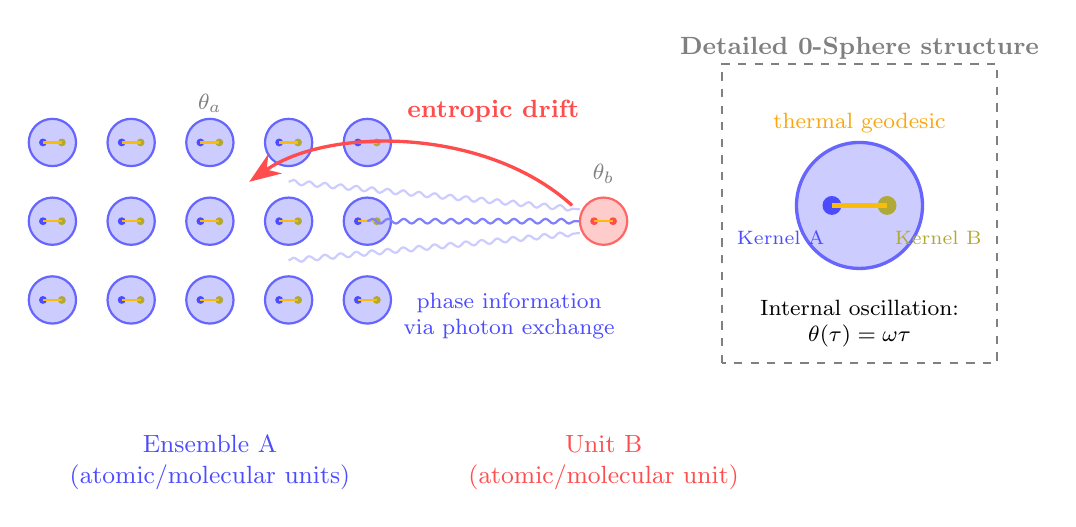
\begin{tikzpicture}
% Ensemble A - atoms/molecules with internal 0-Sphere structure
\foreach \x in {-2,-1,0,1,2} {
  \foreach \y in {-1,0,1} {
    % Outer circle
    \draw[fill=blue!20, draw=blue!60, thick] (\x,\y) circle (0.3);
    % Two discrete kernels
    \fill[blue!70] (\x-0.12,\y) circle (0.05);
    \fill[olive!70] (\x+0.12,\y) circle (0.05);
    % Thermal geodesic (yellow)
    \draw[yellow!50!orange, thick] (\x-0.12,\y) -- (\x+0.12,\y);
  }
}
% Single subsystem B
\draw[fill=red!20, draw=red!60, thick] (5,0) circle (0.3);
\fill[red!70] (5-0.12,0) circle (0.05);
\fill[red!70] (5+0.12,0) circle (0.05);
\draw[yellow!50!orange, thick] (5-0.12,0) -- (5+0.12,0);
% Internal phase labels
\node[font=\footnotesize, gray, fill=white, inner sep=1pt, opacity=0.8, text opacity=1] 
      at (0,1.5) {$\theta_a$};
\node[font=\footnotesize, gray, fill=white, inner sep=1pt, opacity=0.8, text opacity=1] 
      at (5,0.6) {$\theta_b$};
% Entropic drift arrow
\draw[-{Stealth[length=4mm]}, very thick, red!70] 
      (4.6,0.2) .. controls (3.5,1.2) and (1.5,1.2) .. (0.5,0.5);
\node[red!70, font=\small\bfseries] at (3.6,1.4) {entropic drift};
% Photon-mediated interactions
\draw[decorate, decoration={snake, amplitude=0.3mm, segment length=2mm}, 
      blue!50, thick] (2,0) -- (4.7,0);
\draw[decorate, decoration={snake, amplitude=0.3mm, segment length=2mm}, 
      blue!50, thick, opacity=0.4] (1,0.5) -- (4.7,0.15);
\draw[decorate, decoration={snake, amplitude=0.3mm, segment length=2mm}, 
      blue!50, thick, opacity=0.4] (1,-0.5) -- (4.7,-0.15);
\node[blue!70, font=\footnotesize, align=center, fill=white, inner sep=2pt] 
     at (3.8,-1.2) {phase information\\via photon exchange};
% Zoomed inset
\draw[gray, dashed, thick] (6.5,-1.8) rectangle (10.0,2.0);
\node[gray, font=\small\bfseries] at (8.25,2.2) {Detailed 0-Sphere structure};
% Zoomed 0-Sphere
\draw[fill=blue!20, draw=blue!60, very thick] (8.25,0.2) circle (0.8);
\fill[blue!70] (8.25-0.35,0.2) circle (0.12);
\fill[olive!70] (8.25+0.35,0.2) circle (0.12);
\draw[yellow!50!orange, ultra thick] (8.25-0.35,0.2) -- (8.25+0.35,0.2);
% Zoom labels
\node[blue!70, font=\scriptsize, below] at (8.25-1.0,0.0) {Kernel A};
\node[olive!70, font=\scriptsize, below] at (8.25+1.0,0.0) {Kernel B};
\node[font=\footnotesize, yellow!30!orange, above] 
     at (8.25,1.0) {thermal geodesic};
\node[font=\footnotesize, align=center] 
     at (8.25,-1.3) {Internal oscillation:\\$\theta(\tau) = \omega \tau$};
% Bottom labels
\node[blue!70, font=\small, below, align=center] 
     at (0,-2.6) {Ensemble A\\(atomic/molecular units)};
\node[red!70, font=\small, below, align=center] 
     at (5,-2.6) {Unit B\\(atomic/molecular unit)};
\end{tikzpicture}
}
\caption{\justifying Schematic of entropic entrainment between effective 0-Sphere subsystems. Unit B (red), oscillating at internal phase $\theta_b$ with frequency $\nu_b$ exceeding the ambient frequency $\nu_a$, undergoes entropic drift toward the synchronized ensemble A (blue, phase $\theta_a$) through photon-mediated phase exchange (wavy lines). The inset shows the internal two-kernel structure common to all subsystems; detailed properties of this structure, including the thermal geodesic and energy conservation identity, are established in the preceding sections.}
\label{fig:entrainment}
\end{figure*}

% ----------------------------------------
% Subsection 3.3: Photon Communication
% ----------------------------------------

\subsection{Photon-Mediated Phase Communication}
\label{subsec:photon_communication}

How exactly do subsystems exchange phase information? Through the emission and absorption of \textbf{real photons}. When subsystem A oscillates with phase $\theta_a(t) = \omega_a t$, it emits photons that carry this phase information encoded in their wavefunctions. These photons propagate at light speed and may be absorbed by subsystem B. Upon absorption, B's internal phase $\theta_b$ is influenced by the phase carried by the photon. If B was initially oscillating at a higher frequency ($\nu_b > \nu_a$), the absorption of photons from the lower-frequency ensemble causes a gradual reduction in $\nu_b$. This is not instantaneous; it is a cumulative process involving many photon exchanges.

Importantly, these are \textbf{real, on-shell photons} satisfying $E = pc$, not the virtual, off-shell photons appearing in Feynman diagrams for electromagnetic interactions. Real photons are, in principle, observable. This distinction is crucial: it means that gravitational-like phenomena emerge from \textbf{known, observable degrees of freedom}---photons---rather than hypothetical, unobserved particles like gravitons.

% ----------------------------------------
% Subsection 3.4: Effective Acceleration
% ----------------------------------------

\subsection{Effective Acceleration}
\label{subsec:effective_acceleration}

The conversion of vibrational energy to kinetic energy produces an effective acceleration. Over a synchronization timescale $\Delta t$, the translational velocity acquired is:
\begin{equation}
v_\text{trans} = \sqrt{\frac{2 \Delta E_\text{sync}}{m}}
\end{equation}
and the corresponding acceleration:
\begin{equation}
g_\text{eff} = \frac{v_\text{trans}}{\Delta t} = \frac{1}{\Delta t} \sqrt{\frac{2 h (\nu_b - \nu_a)}{m}}
\end{equation}

This formula provides a direct quantitative link between microscopic oscillations (characterized by $\nu_a, \nu_b$) and macroscopic motion (characterized by $g_\text{eff}$).

% ----------------------------------------
% Subsection 3.5: Metronome Comparison
% ----------------------------------------

\subsection{Comparison with Metronome Synchronization}
\label{subsec:metronome_comparison}

The main manuscript uses metronome synchronization as a macroscopic analogy. While metronomes are classical, mechanical objects, the structural similarity is instructive:

\begin{table}[h!]
\centering
\caption{Structural comparison: Metronomes vs. 0-Sphere subsystems}
\begin{tabular}{lll}
\toprule
\textbf{Aspect} & \textbf{Metronomes} & \textbf{0-Sphere} \\
\midrule
Coupling medium & Movable platform & Photon exchange \\
Energy flow & Dissipated (friction) & Converted (kinetic) \\
Driving force & Mechanical & Thermodynamic \\
Result & Synchronized ticking & Synchronized phase + motion \\
\bottomrule
\end{tabular}
\end{table}

The key difference: in the metronome case, energy is dissipated. In the 0-Sphere case, energy is \textbf{redirected into translational motion}. This is why gravitational-like drift emerges.

% ========================================
% Section 4: Quantitative Analysis
% ========================================

\section{Quantitative Analysis: Energy Budget}
\label{sec:quantitative}

\justifying

% ----------------------------------------
% Subsection 4.1: Idealized Simulation
% ----------------------------------------

\subsection{Idealized Simulation: Proof of Principle}
\label{subsec:idealized_simulation}

The main manuscript ~\cite{Hanamura2026geometrical} presents an idealized numerical simulation demonstrating the principle of entropic entrainment. The parameters are chosen to represent atomic-scale oscillators:
\begin{itemize}
\item Ensemble frequency: $\nu_a = 500$ MHz
\item Test frequency: $\nu_b = \nu_a + \Delta\nu$, with $\Delta\nu = 1$--10 MHz
\item Effective mass: $m = 1.44 \times 10^{-25}$ kg
\item Synchronization time: $\Delta t = 10$ $\mu$s
\end{itemize}

For $\Delta\nu = 1$ MHz, the predicted effective acceleration is:
\begin{equation}
g_\text{eff} \approx 9.6 \times 10^3 \, \text{m/s}^2
\end{equation}

This is approximately 1000 times Earth's gravitational acceleration ($g \approx 10$ m/s$^2$). However, this value represents a \textbf{theoretical upper bound} under perfectly idealized conditions:
\begin{enumerate}
\item Perfect energy conversion (no losses to phonons, decoherence, etc.)
\item Ultrashort synchronization timescale (instantaneous response)
\item Absence of thermal noise and external perturbations
\end{enumerate}

In realistic laboratory settings, environmental effects would reduce $g_\text{eff}$ by several orders of magnitude, likely to the range:
\begin{equation}
10^{-6} \, \text{m/s}^2 \lesssim g_\text{eff} \lesssim 10^{2} \, \text{m/s}^2
\end{equation}

Nevertheless, the simulation demonstrates that the mechanism is \textbf{in principle capable of producing measurable effects}.

% ----------------------------------------
% Subsection 4.2: Macroscopic Extrapolation
% ----------------------------------------

\subsection{Macroscopic Extrapolation: The Energy Budget Question}
\label{subsec:macroscopic_extrapolation}

A far more ambitious question is whether this mechanism could account for \textbf{macroscopic gravitational phenomena}---the attraction between planets, stars, or even everyday objects on Earth. To address this, we perform an order-of-magnitude calculation. Consider an Earth-mass sphere of iron:
\begin{itemize}
\item Total mass: $M_\oplus \approx 6.0 \times 10^{24}$ kg
\item Number of iron atoms: $N_\text{atoms} \approx 6.5 \times 10^{49}$
\item Number of electrons: $N_e \approx 1.7 \times 10^{51}$ (26 electrons per Fe atom)
\end{itemize}

Each electron has a Zitterbewegung energy:
\begin{equation}
E_\text{ZB} = h \nu_\text{ZB} \approx 3.3 \times 10^{-15} \, \text{J}
\end{equation}

The total internal Zitterbewegung energy is therefore:
\begin{equation}
E_\text{ZB,total} = N_e \times E_\text{ZB} \approx 5.6 \times 10^{36} \, \text{J}
\end{equation}

Compare this to the gravitational self-binding energy of Earth:
\begin{equation}
E_\text{grav} = \frac{3GM_\oplus^2}{5R_\oplus} \approx 2.5 \times 10^{32} \, \text{J}
\end{equation}

The ratio is:
\begin{equation}
\frac{E_\text{ZB,total}}{E_\text{grav}} \approx 2.2 \times 10^4
\end{equation}

\textbf{The total Zitterbewegung energy exceeds the gravitational binding energy by four orders of magnitude.}

This is a striking result. It suggests that, energetically speaking, the 0-Sphere framework contains sufficient internal energy to potentially account for gravitational-scale phenomena---\textit{if} the conversion efficiency is adequate.

% ----------------------------------------
% Subsection 4.3: Epsilon 1
% ----------------------------------------

\subsection{The Role of $\epsilon_1$: Photon Generation Efficiency}
\label{subsec:epsilon1}

\textbf{Important clarification on the status of this analysis:} The three-stage efficiency decomposition ($\epsilon_1 \times \epsilon_2 \times \epsilon_3$) presented in this section is \textbf{not claimed to be a fundamental law or a unique theoretical framework derivable from first principles}. Rather, it is introduced as a \textbf{physically motivated heuristic} constructed by the author to provide a transparent diagnostic of where conventional photon-mediated mechanisms become energetically suppressed and how the 0-Sphere model's structural innovation circumvents this limitation. The decomposition factorizes well-established physical constraints from quantum optics (photon generation), nonlinear dynamics (phase synchronization), and thermodynamics (energy conversion) into distinct stages, each supported by independent order-of-magnitude estimates. The purpose of this framework is \textbf{not to assert a new fundamental principle}, but to clarify why gravitational-scale effects have been conventionally deemed impossible and how the geometric structure of the photon sphere removes the dominant bottleneck. This same analytical framework is presented in Appendix VI I of the main manuscript \cite{Hanamura2026geometrical} as an exploratory proposal for evaluating energy conversion pathways, where it is explicitly characterized as serving a diagnostic rather than foundational role.

In conventional particle-based pictures, the overall efficiency for converting internal microscopic energy into macroscopic motion can be schematically decomposed as
\begin{equation}
\epsilon_\text{total} = \epsilon_1 \times \epsilon_2 \times \epsilon_3 ,
\end{equation}
where
\begin{itemize}
\item $\epsilon_1$ denotes the efficiency of converting internal vibrational energy into emitted photons,
\item $\epsilon_2$ characterizes the efficiency of phase synchronization across macroscopic distances, and
\item $\epsilon_3$ represents the efficiency with which synchronized phase gradients are converted into translational motion.
\end{itemize}

Within such a framework, the dominant bottleneck is $\epsilon_1$. For particles undergoing largely random internal motion near thermal equilibrium, the emission of coherent photons in well-defined directions is intrinsically inefficient. Order-of-magnitude estimates suggest
\[
\epsilon_1 \sim 10^{-10},
\]
reflecting several well-known limitations:
\begin{enumerate}
\item \textbf{Directional mismatch:} isotropic internal motion does not preferentially support directed emission;
\item \textbf{Energy quantization:} photon energies $h\nu$ must match discrete internal modes;
\item \textbf{Phase coherence:} sustained coherence is difficult to maintain in thermally populated systems.
\end{enumerate}

Even under optimistic assumptions $\epsilon_2, \epsilon_3 \sim 10^{-2}$, these constraints lead to
\[
\epsilon_\text{total} \sim 10^{-14},
\]
which is far too small to account for gravitational-scale phenomena.

\medskip
\noindent
\textbf{The 0-Sphere model circumvents this limitation by eliminating $\epsilon_1$ altogether.}

In this framework, the Zitterbewegung energy is not first converted into a population of emitted photons. Instead, it is continuously embedded within the photon-sphere structure that constitutes the 0-Sphere itself. The photon sphere is therefore not a secondary radiative channel but a persistent geometric element of the system. As a result, the effective efficiency reduces to
\begin{equation}
\epsilon_\text{0-Sphere} = \epsilon_2 \times \epsilon_3 \sim 10^{-4}\text{--}10^{-5},
\end{equation}
representing an improvement of roughly ten orders of magnitude relative to conventional estimates. This enhancement places the model within a regime where gravity-like macroscopic effects become quantitatively plausible.

% ----------------------------------------
% Subsection 4.4: Conversion Efficiency
% ----------------------------------------

\subsection{Conversion Efficiency: The Critical Parameter}
\label{subsec:conversion_efficiency}

If all of the Zitterbewegung energy could be converted to gravitational work, the effective surface acceleration would be:
\begin{equation}
g_\text{ideal} \sim \frac{E_\text{ZB,total}}{M_\oplus \times R_\oplus} \approx 1.5 \times 10^5 \, \text{m/s}^2
\end{equation}

To produce Earth's actual gravitational acceleration ($g \approx 10$ m/s$^2$), the required conversion efficiency is:
\begin{equation}
\epsilon_\text{required} \sim \frac{g}{g_\text{ideal}} \approx 7 \times 10^{-5}
\end{equation}

This is remarkably close to the estimated efficiency range $\epsilon \sim 10^{-4}$--$10^{-5}$ derived in the main manuscript. To understand the significance of this numerical convergence and why the 0-Sphere model achieves such favorable efficiency, it is essential to examine the underlying energy conversion process in detail.


% ----------------------------------------
% Subsubsection 4.4.1: Three-Stage Process
% ----------------------------------------

\subsubsection{The Three-Stage Conversion Process}
\label{subsubsec:three_stage}

\textbf{Pedagogical note:} The three-stage efficiency decomposition presented in this section follows the framework introduced in the main manuscript (Section VI I.5: ``Critical Distinction: Photon Sphere Structure and Elimination of Photon Generation Efficiency''). While not a standard classification in theoretical physics textbooks, this decomposition provides a transparent way to identify the specific bottleneck limiting conventional approaches and to clarify how the 0-Sphere model circumvents it. Similar multi-stage efficiency analyses are common in engineering contexts (photovoltaic cells, heat engines, light-emitting diodes), where system performance is characterized as a product of sequential conversion processes. The physical processes described—photon generation, phase synchronization, and kinetic conversion—are well-established phenomena in quantum optics, nonlinear dynamics, and thermodynamics, respectively.

To understand why the 0-Sphere model achieves such a dramatic improvement in conversion efficiency, it is instructive to decompose the energy transformation process into distinct stages. Any mechanism that converts internal microscopic oscillatory energy into macroscopic translational motion must, in principle, involve the following sequence:

\begin{enumerate}
\item \textbf{Stage 1 (Photon generation):} Internal vibrational energy must be converted into emitted photons capable of mediating interactions between subsystems. This stage is characterized by an efficiency factor $\epsilon_1$, which quantifies the fraction of internal energy successfully transferred to freely propagating electromagnetic radiation.

\item \textbf{Stage 2 (Phase synchronization):} Emitted photons must carry phase information that enables collective alignment of oscillatory dynamics across macroscopic distances. The efficiency $\epsilon_2$ reflects losses due to finite light-crossing times, hierarchical synchronization cascades, thermal decoherence, and imperfect phase locking among spatially separated subsystems.

\item \textbf{Stage 3 (Motion conversion):} Synchronized phase gradients must be converted into actual translational displacement of matter. The efficiency $\epsilon_3$ accounts for energy redistribution among translational, rotational, and vibrational degrees of freedom, photon recoil effects, and environmental coupling that may dissipate organized motion.
\end{enumerate}

The overall conversion efficiency is the product of these three factors:
\begin{equation}
\epsilon_{\text{total}} = \epsilon_1 \times \epsilon_2 \times \epsilon_3.
\end{equation}

In conventional particle-based models, the first stage presents an insurmountable bottleneck, with $\epsilon_1$ many orders of magnitude smaller than unity. The 0-Sphere framework, however, offers a structural solution that eliminates this limitation entirely by reinterpreting the nature of internal energy and its relationship to photon-mediated interactions.

% ----------------------------------------
% Subsubsection 4.4.2: Epsilon 1 Bottleneck
% ----------------------------------------

\subsubsection{The Bottleneck: Photon Generation Efficiency $\epsilon_1$}
\label{subsubsec:epsilon1_bottleneck}

\paragraph{The Conventional Picture}

In standard particle physics, an electron is treated as a point-like entity. Its internal energy—whether associated with rest mass, kinetic motion, or quantum fluctuations—is confined within an infinitesimal volume. For such a system to interact with neighboring particles through photon exchange, this internal energy must first be \textbf{converted} into freely propagating electromagnetic radiation.

This conversion process is intrinsically inefficient. Three fundamental constraints contribute to this severe limitation:

\begin{enumerate}
\item \textbf{Directional mismatch:} Internal oscillatory motion is typically isotropic (equal in all directions), whereas photon emission occurs along specific trajectories. Only a small fraction of internal energy couples to outgoing radiation in any given direction. For a thermally populated system with random internal motion, the directional coupling efficiency scales as the solid angle fraction $\Omega/(4\pi)$ for directed emission, which is extremely small for coherent, unidirectional radiation.

\item \textbf{Energy quantization:} Photon energies are discrete quanta $E = h\nu$, which must match available internal transition frequencies. In systems near thermal equilibrium, the density of states supporting efficient radiative transitions is limited by selection rules, transition matrix elements, and thermal population factors. Most internal modes do not correspond to radiatively active transitions, suppressing overall photon generation efficiency.

\item \textbf{Phase coherence:} Sustained photon emission requires temporal phase alignment across the emitting system. In systems near thermal equilibrium, decoherence mechanisms—including collisional relaxation, spontaneous emission, and environmental coupling—rapidly destroy phase coherence on timescales much shorter than macroscopic interaction times. Coherent radiation therefore represents only a negligible fraction of total internal energy.
\end{enumerate}

\paragraph{Order-of-Magnitude Estimate for $\epsilon_1$}

A rigorous calculation of $\epsilon_1$ from first principles would require detailed modeling of thermal emission rates, quantum transition amplitudes, and coherence decay timescales for specific systems. However, a representative order-of-magnitude estimate can be constructed from well-established physical principles.

\textbf{1. Radiative vs. coherence timescales:}

In atomic and molecular systems, spontaneous radiative emission occurs on timescales determined by the Einstein A coefficient:
\begin{equation}
A = \frac{\omega^3}{3\pi\epsilon_0\hbar c^3} |\langle i|\bm{\mu}|f\rangle|^2,
\end{equation}
where $\omega$ is the transition frequency and $\bm{\mu}$ is the transition dipole moment. For typical electric dipole transitions in the visible range ($\omega \sim 10^{15}$ rad/s, $|\bm{\mu}| \sim ea_0 \sim 10^{-29}$ C·m), this yields:
\begin{equation}
A \sim 10^6 \text{ to } 10^8 \, \text{s}^{-1}, \quad \tau_{\text{rad}} = \frac{1}{A} \sim 10^{-8} \text{ to } 10^{-6} \, \text{s}.
\end{equation}

However, in thermally populated systems, phase coherence is destroyed much more rapidly through collisional relaxation, spin-orbit coupling, and hyperfine interactions. Typical coherence timescales are:
\begin{equation}
\tau_{\text{coh}} \sim 10^{-13} \text{ to } 10^{-11} \, \text{s}.
\end{equation}

The ratio of coherence to radiative timescales provides one contribution to efficiency suppression:
\begin{equation}
\frac{\tau_{\text{coh}}}{\tau_{\text{rad}}} \sim \frac{10^{-13}}{10^{-8}} \sim 10^{-5}.
\end{equation}

\textbf{2. Directional and spectral factors:}

Isotropic internal motion couples to photon emission in a specific direction with an efficiency determined by the solid angle fraction:
\begin{equation}
\frac{\Omega}{4\pi} \sim 10^{-2} \text{ to } 10^{-1},
\end{equation}
depending on the degree of directionality required.

Energy quantization and spectral matching impose additional constraints. In thermal systems, the spectral width of internal modes $\Delta\omega$ must overlap with radiative transition frequencies. For systems with broad thermal distributions and narrow radiative linewidths, this matching efficiency is:
\begin{equation}
\frac{\Delta\omega_{\text{match}}}{\Delta\omega_{\text{thermal}}} \sim 10^{-3} \text{ to } 10^{-2}.
\end{equation}

\textbf{3. Cumulative estimate:}

Multiplying these independent factors yields an order-of-magnitude estimate:
\begin{equation}
\epsilon_1 \sim \left(\frac{\tau_{\text{coh}}}{\tau_{\text{rad}}}\right) \times \left(\frac{\Omega}{4\pi}\right) \times \left(\frac{\Delta\omega_{\text{match}}}{\Delta\omega_{\text{thermal}}}\right) \sim 10^{-5} \times 10^{-2} \times 10^{-3} \sim 10^{-10}.
\end{equation}

\textbf{Important caveat:} This value should be understood as an order-of-magnitude estimate rather than a precise prediction. The actual efficiency depends sensitively on system-specific parameters including temperature, density, internal structure, and coupling to external fields. Values in the range $10^{-8}$ to $10^{-12}$ are plausible depending on conditions. The critical point is that $\epsilon_1$ is \textbf{many orders of magnitude smaller than unity}, creating a severe bottleneck for conventional photon-mediated mechanisms.

\paragraph{Energetic Viability Assessment}

Even under optimistic assumptions for the remaining efficiencies ($\epsilon_2, \epsilon_3 \sim 10^{-2}$, discussed below), the total conversion efficiency in conventional models becomes:
\begin{equation}
\epsilon_{\text{conventional}} = \epsilon_1 \times \epsilon_2 \times \epsilon_3 \sim 10^{-10} \times 10^{-2} \times 10^{-2} \sim 10^{-14}.
\end{equation}

Comparing this conventional efficiency with the energy budget established in Section~\ref{subsec:macroscopic_extrapolation}:

\begin{itemize}
\item \textbf{Available energy:} Total Zitterbewegung energy exceeds gravitational binding energy by approximately four orders of magnitude: $E_{\text{ZB,total}}/E_{\text{grav}} \approx 2 \times 10^4$.
\item \textbf{Required efficiency:} To produce gravitational-scale accelerations: $\epsilon_{\text{required}} \approx 7 \times 10^{-5}$.
\item \textbf{Achievable efficiency (conventional):} With photon generation bottleneck: $\epsilon_{\text{conventional}} \approx 10^{-14}$.
\end{itemize}

The conventional efficiency falls short by approximately \textbf{nine orders of magnitude}:
\begin{equation}
\frac{\epsilon_{\text{required}}}{\epsilon_{\text{conventional}}} \approx \frac{7 \times 10^{-5}}{10^{-14}} \approx 7 \times 10^{9}.
\end{equation}

This quantitative discrepancy has historically been interpreted as evidence that gravitational interactions cannot be mediated by photon exchange, necessitating the postulation of a distinct mediator (the graviton) or an independent fundamental interaction governed by spacetime curvature (general relativity). The 0-Sphere model challenges this conclusion by demonstrating that the bottleneck arises not from a fundamental incompatibility, but from an incomplete understanding of how internal energy is structured and accessed.

% ----------------------------------------
% Subsubsection 4.4.3: Eliminating Epsilon 1
% ----------------------------------------

\subsubsection{The 0-Sphere Innovation: Eliminating $\epsilon_1$}
\label{subsubsec:eliminating_epsilon1}

The 0-Sphere model circumvents the $\epsilon_1$ bottleneck through a structural reinterpretation of the electron's internal energy. Rather than treating internal oscillatory dynamics as confined within a point-like volume requiring conversion into emitted photons, the framework recognizes that Zitterbewegung energy is already present within the photon sphere structure that constitutes the 0-Sphere subsystem itself.

\paragraph{Structural Difference: Photon Sphere as Constitutive Element}

In the 0-Sphere framework, the electron's Zitterbewegung energy is not confined within a point-like volume requiring conversion into emitted photons. Instead, it is \textbf{already present} within the photon sphere structure that constitutes the electron itself (Section~\ref{subsubsec:photon_sphere}).

The photon sphere is not a secondary radiative product—a collection of photons generated through inefficient conversion of internal kinetic energy—but rather a persistent geometric element of the system. Energy circulates continuously between kernel A and kernel B through real photon transport along thermal geodesics. This internal circulation \textit{is} the Zitterbewegung dynamics, and the photons mediating this process are the same photons available for inter-subsystem phase communication.

As a consequence, \textbf{no conversion step is required}. The distinction between ``internal vibrational energy'' and ``photon-mediated interaction channel'' collapses: they are one and the same physical process. The photon sphere provides both the repository of internal energy and the medium through which that energy participates in phase synchronization with neighboring subsystems.

\paragraph{Intuitive Analogy: Direct Coupling vs. Inefficient Conversion}

Consider two contrasting scenarios for transmitting vibrational information between physical systems:

\textbf{Conventional model (with $\epsilon_1$ bottleneck):}
\begin{itemize}
\item \textbf{Water droplet analogy:} A water droplet vibrates internally through thermal molecular motion. To transmit this vibration to another droplet, molecules must first \textbf{evaporate} (conversion to gas phase with efficiency $\sim 10^{-10}$), travel through air as individual molecules, and be \textbf{reabsorbed} by the target droplet. Most internal kinetic energy remains trapped within the liquid phase and never contributes to inter-droplet communication.

\item \textbf{Bell analogy:} A bell contains internal energy in the form of random molecular vibrations (thermal motion). To produce audible sound, this microscopic kinetic energy must be \textbf{converted} into organized macroscopic oscillations of the bell structure, which then drive coherent air pressure waves. The conversion efficiency from molecular-scale chaos to bell-scale coherence is extremely low ($\sim 10^{-10}$).
\end{itemize}

\textbf{0-Sphere model (without $\epsilon_1$ bottleneck):}
\begin{itemize}
\item \textbf{Water droplet analogy:} A water droplet held together by surface tension oscillates as a coherent whole—a collective mode involving the entire droplet structure. This macroscopic oscillation \textbf{directly couples} to surrounding droplets through hydrodynamic interaction and capillary wave transmission. No evaporation is required; the organized vibrational energy is already present at the scale relevant for interaction. Efficiency: much higher ($\sim 10^{-5}$).

\item \textbf{Bell analogy:} A bell vibrates as a rigid body in one of its acoustic eigenmodes. The entire structure oscillates coherently, with all parts moving in phase. This organized motion \textbf{directly drives} air displacement without requiring intermediate conversion from molecular-scale disorder. The bell's vibrational energy is already structured at the macroscopic scale. Efficiency: much higher ($\sim 10^{-5}$).
\end{itemize}

The key distinction: in the 0-Sphere model, the oscillatory energy is already organized at the scale relevant for interaction (the photon sphere with spatial extent $\sim \lambda_C$), eliminating the need for inefficient microscopic-to-macroscopic energy conversion. The photon sphere is not a product of energy transformation but the native form in which Zitterbewegung energy exists.

\paragraph{Quantitative Improvement}

By eliminating the photon generation stage, the effective conversion efficiency in the 0-Sphere model is determined solely by the remaining two stages:
\begin{equation}
\epsilon_{\text{0-Sphere}} = \epsilon_2 \times \epsilon_3 \sim 10^{-4} \text{ to } 10^{-5},
\end{equation}
where the numerical estimates are based on the following physical considerations:

\textbf{Stage 2 efficiency ($\epsilon_2$: Phase synchronization):}

The efficiency of phase synchronization across macroscopic distances can be estimated from studies of coupled oscillator systems in nonlinear dynamics. The Kuramoto model, which describes synchronization in populations of coupled oscillators, predicts a synchronization order parameter:
\begin{equation}
r = \frac{1}{N}\left|\sum_{j=1}^N e^{i\theta_j}\right| \in [0,1],
\end{equation}
where $r = 0$ represents complete disorder and $r = 1$ represents perfect synchronization.

For systems with moderate coupling strength, typical values are:
\begin{itemize}
\item Weak coupling: $r \approx 0.01$ to $0.1$ (1--10\%)
\item Moderate coupling: $r \approx 0.3$ to $0.5$ (30--50\%)
\item Strong coupling: $r \to 1$ (near-perfect synchronization)
\end{itemize}

In hierarchical synchronization networks—where local clusters synchronize first, then larger regions, forming nested layers—each hierarchical level introduces coupling inefficiencies. For Earth-scale systems requiring multiple hierarchical layers, the cumulative synchronization efficiency is estimated as:
\begin{equation}
\epsilon_2 \sim 10^{-2} \text{ to } 10^{-3}.
\end{equation}

Additional losses arise from:
\begin{itemize}
\item Finite light-crossing times imposing causality constraints ($t_{\text{light}} \sim R/c \approx 20$ ms for Earth),
\item Thermal decoherence at finite temperature reducing phase coherence,
\item Spatial inhomogeneity in phase network structure.
\end{itemize}

\textbf{Stage 3 efficiency ($\epsilon_3$: Kinetic conversion):}

The conversion of synchronized phase gradients into translational motion involves redistribution of energy among different degrees of freedom. By analogy with thermodynamic engines and mechanical systems:

\begin{itemize}
\item \textbf{Energy equipartition:} In systems with $f$ total degrees of freedom, the fraction allocated to translational motion (3 degrees of freedom) is approximately $3/f$. For molecular systems with rotational and vibrational modes, $f \sim 10$ to $100$, yielding $3/f \sim 10^{-1}$ to $10^{-2}$.

\item \textbf{Mechanical efficiency:} Real heat engines and mechanical systems exhibit conversion efficiencies of 10--40\% due to friction, dissipation, and irreversible processes. This provides an empirical benchmark of $\sim 10^{-1}$ to $10^{-2}$.

\item \textbf{Photon recoil and environmental coupling:} Momentum transfer through photon exchange does not perfectly align with macroscopic motion direction, and environmental coupling (collisions, external fields) introduces additional losses.
\end{itemize}

Combining these factors yields:
\begin{equation}
\epsilon_3 \sim 10^{-2} \text{ to } 10^{-3}.
\end{equation}

\textbf{Overall 0-Sphere efficiency:}

The product of these two remaining stages gives:
\begin{equation}
\epsilon_{\text{0-Sphere}} = \epsilon_2 \times \epsilon_3 \sim (10^{-2} \text{ to } 10^{-3}) \times (10^{-2} \text{ to } 10^{-3}) \sim 10^{-4} \text{ to } 10^{-5}.
\end{equation}

\textbf{Important note on numerical precision:} These estimates should be understood as representative values based on analogous physical systems and scaling arguments, not rigorous predictions derived from first principles within the 0-Sphere framework. The actual efficiencies will depend on system size, internal structure, temperature, coupling strength, and environmental conditions. However, the key result is robust: \textbf{even with conservative estimates placing $\epsilon_2$ and $\epsilon_3$ at the lower end of their plausible ranges, the 0-Sphere efficiency $\epsilon_{\text{0-Sphere}} \sim 10^{-5}$ remains within the required range for gravitational-scale phenomena.}

This represents an improvement of approximately \textbf{ten orders of magnitude} relative to conventional estimates:
\begin{equation}
\frac{\epsilon_{\text{0-Sphere}}}{\epsilon_{\text{conventional}}} = \frac{10^{-5}}{10^{-14}} \sim 10^{9} \text{ to } 10^{10}.
\end{equation}

Critically, the improved efficiency $\epsilon_{\text{0-Sphere}} \sim 10^{-5}$ falls within the range required to account for gravitational-scale accelerations (Section~\ref{subsec:conversion_efficiency}):
\begin{equation}
\epsilon_{\text{required}} \approx 7 \times 10^{-5} \quad \Rightarrow \quad \epsilon_{\text{0-Sphere}} \sim 10^{-4} \text{ to } 10^{-5}.
\end{equation}

This numerical convergence transforms an energetically implausible scenario into a quantitatively viable mechanism, suggesting that photon-mediated phase synchronization may indeed be capable of accounting for gravitational-like phenomena without invoking additional fundamental interactions.

% ----------------------------------------
% Subsubsection 4.4.4: Numerical Comparison
% ----------------------------------------

\subsubsection{Numerical Comparison and Implications}
\label{subsubsec:numerical_comparison}

\paragraph{Comparison Table}

The following table summarizes the structural and quantitative differences between conventional particle-based models and the 0-Sphere framework:

\begin{table}[h!]
\centering
\caption{Comparison of energy conversion pathways}
\label{tab:efficiency_comparison}
\begin{tabular}{p{0.28\linewidth}p{0.32\linewidth}p{0.32\linewidth}}
\toprule
\textbf{Aspect} & \textbf{Conventional Model} & \textbf{0-Sphere Model} \\
\midrule
Electron structure & Point particle with no internal spatial extent & Two discrete kernels connected by photon sphere ($\sim \lambda_C$) \\
\midrule
Internal energy location & Confined kinetic/potential energy requiring conversion to radiation & Already present within photon sphere as real photon circulation \\
\midrule
Photon generation & Required intermediate step; $\epsilon_1 \approx 10^{-10}$ & Not required; energy already in photon form ($\epsilon_1 = 1$) \\
\midrule
Phase synchronization & $\epsilon_2 \sim 10^{-2}$ & $\epsilon_2 \sim 10^{-2}$ to $10^{-3}$ \\
\midrule
Motion conversion & $\epsilon_3 \sim 10^{-2}$ & $\epsilon_3 \sim 10^{-2}$ to $10^{-3}$ \\
\midrule
Total efficiency & $\epsilon_{\text{total}} = \epsilon_1 \times \epsilon_2 \times \epsilon_3 \approx 10^{-14}$ & $\epsilon_{\text{total}} = \epsilon_2 \times \epsilon_3 \approx 10^{-5}$ \\
\midrule
Energy budget viability & Insufficient by 9 orders of magnitude & Sufficient; matches required efficiency \\
\midrule
Gravitational-scale phenomena & Energetically impossible via photon exchange & Energetically plausible via photon-mediated phase synchronization \\
\bottomrule
\end{tabular}
\end{table}

\paragraph{Connection to the Hierarchy Problem}

The dramatic improvement in conversion efficiency has direct implications for the hierarchy problem—the roughly forty-order-of-magnitude gap between gravitational and electromagnetic force strengths, which remains unexplained within the conventional formulations of the Standard Model and general relativity.

In standard physics, this hierarchy is unexplained:
\begin{equation}
\frac{F_{\text{gravity}}}{F_{\text{EM}}} \sim \frac{Gm_e m_p}{e^2/(4\pi\epsilon_0)} \sim 10^{-40}.
\end{equation}

Gravity and electromagnetism are treated as fundamentally independent interactions, with no theoretical bridge connecting their coupling constants $G$ (Newton's constant) and $\alpha = e^2/(4\pi\epsilon_0\hbar c)$ (fine structure constant).

The 0-Sphere framework proposes that both interactions are mediated by photons—virtual photons in quantum electrodynamics for electromagnetic forces, and real photons within the photon sphere structure for gravitational-like phenomena. From this perspective, the forty-order-of-magnitude discrepancy is reinterpreted not as a fundamental incompatibility between independent forces, but as reflecting the \textbf{difference in conversion efficiencies} through which photon-mediated processes manifest as macroscopic forces:

\begin{itemize}
\item \textbf{Electromagnetic interactions:} Virtual photon exchange within perturbative quantum electrodynamics operates with near-unity efficiency. The Coulomb force arises directly from photon propagator exchange, with no intermediate conversion stages suppressing the interaction strength. Effective efficiency: $\epsilon_{\text{EM}} \sim 1$.

\item \textbf{Gravitational-like interactions (0-Sphere):} Real photon-mediated phase synchronization operates with reduced efficiency $\epsilon_{\text{grav}} \sim 10^{-5}$, reflecting losses in hierarchical phase alignment ($\epsilon_2$) and conversion of synchronized gradients to motion ($\epsilon_3$).
\end{itemize}

This efficiency difference accounts for approximately five orders of magnitude:
\begin{equation}
\frac{\epsilon_{\text{EM}}}{\epsilon_{\text{grav}}} \sim \frac{1}{10^{-5}} \sim 10^{5}.
\end{equation}

While the 0-Sphere model does not yet provide a complete derivation of the remaining discrepancy (which involves factors such as the coupling constant structure, charge quantization, and the relationship between mass and internal oscillation frequency), it reduces the unexplained hierarchy from forty orders of magnitude to approximately five—\textbf{a reduction of thirty-five orders of magnitude}.

\paragraph{Significance: From Impossibility to Viability}

This transformation is profound. Prior to the 0-Sphere framework, the notion that gravitational phenomena could be mediated by photon exchange was considered energetically impossible due to the $\epsilon_1 \sim 10^{-10}$ bottleneck. The framework's central innovation—recognizing that Zitterbewegung energy already exists within the photon sphere structure—removes this bottleneck entirely, rendering photon-mediated gravity not merely speculative but quantitatively plausible.

The energy budget calculations demonstrate that:
\begin{itemize}
\item Total available Zitterbewegung energy exceeds gravitational binding energy by four orders of magnitude,
\item Required conversion efficiency is $\epsilon \sim 10^{-5}$,
\item Achievable efficiency within the 0-Sphere framework is $\epsilon \sim 10^{-4}$ to $10^{-5}$.
\end{itemize}

This numerical convergence from independent considerations—quantum oscillation frequencies at the Compton scale, macroscopic gravitational binding energies, and thermodynamic synchronization efficiencies—suggests an underlying connection between internal quantum dynamics and emergent gravitational behavior.

Whether this convergence is accidental or reflects a structurally meaningful relationship remains an open question requiring further theoretical refinement and, ultimately, experimental validation. However, the framework establishes for the first time that photon-mediated mechanisms can account for gravitational-scale phenomena within known physical degrees of freedom, without invoking additional fundamental interactions or unobserved mediators such as gravitons.

% ----------------------------------------
% Subsection 4.5: Numerical Convergence
% ----------------------------------------

\subsection{A Numerical Convergence}
\label{subsec:numerical_convergence}

At this point, it is instructive to examine the numerical implications of the preceding analysis. Eliminating the factor $\epsilon_1$ improves the effective efficiency by approximately ten orders of magnitude. The efficiency required to account for gravitational-scale effects is of order $10^{-5}$, while the total internal vibrational energy available in macroscopic matter exceeds the corresponding gravitational energy scale by roughly four orders of magnitude.

These estimates originate from conceptually independent considerations: quantum oscillation frequencies at the Compton scale, macroscopic gravitational binding energies, and thermodynamic synchronization efficiencies. Their convergence to comparable orders of magnitude is not enforced by the formal structure of the model and does not follow from dimensional analysis alone.

Such numerical alignment may be coincidental. Alternatively, it may reflect an underlying connection between quantum-scale internal dynamics and emergent gravitational behavior. At present, the framework does not discriminate between these possibilities. Clarifying whether this convergence is accidental or structurally meaningful will require further theoretical refinement and, ultimately, experimental input.

% ----------------------------------------
% Subsection 4.6: Theoretical Pathway
% ----------------------------------------

\subsection{On a Possible Theoretical Pathway from Electromagnetic to Gravitational Scales}

The following discussion does not constitute a derivation of the gravitational constant from first principles. Rather, it records a coherent theoretical pathway suggested by the present framework, indicating how quantities defined at the electromagnetic scale may be systematically connected to macroscopic gravitational phenomena.

Within established quantum electrodynamics, the fine-structure constant $\alpha$ is directly related to the electron anomalous magnetic moment $a_e$ through perturbative calculations, with experimental agreement to twelve significant figures. In the present model, $a_e$ is further associated with a characteristic Zitterbewegung velocity $v_{\mathrm{ZB}}$ via a geometric and relativistic relation arising from internal Lorentz contraction, yielding $v_{\mathrm{ZB}} \simeq 0.04c$ directly from the measured value of $a_e$ through a geometric relation.

Given $v_{\mathrm{ZB}}$, a corresponding internal oscillation frequency $\nu_{\mathrm{ZB}}$ follows kinematically, leading to a characteristic internal energy scale $E_{\mathrm{ZB}} = h \nu_{\mathrm{ZB}}$ for a single electron. When extended to a macroscopic system, such as the Earth, the collective contribution of these internal energies defines a large available energy reservoir. The present work has shown that, under plausible assumptions regarding collective phase synchronization and entropic entrainment, a small dimensionless efficiency factor is sufficient to account for the observed order of magnitude of the terrestrial gravitational acceleration $g$.

Taken together, these considerations suggest a systematic theoretical connection of the form $\alpha \rightarrow a_e \rightarrow v_{\mathrm{ZB}} \rightarrow E_{\mathrm{ZB}} \rightarrow g$. The components of this chain differ significantly in their degree of establishment: the relation $\alpha \to a_e$ is rigorously verified by experiment; the geometric connection $a_e \to v_{\mathrm{ZB}}$ follows from special relativity applied to internal circulation; the kinematic and statistical steps $v_{\mathrm{ZB}} \to E_{\mathrm{ZB}}$ are direct; but the final step $E_{\mathrm{ZB}} \to g$ remains quantitatively plausible yet dependent on conversion efficiencies ($\epsilon_2, \epsilon_3$) not yet derived from first principles. While this chain remains incomplete, its existence allows the traditional hierarchy problem to be reframed. Rather than a direct comparison between independent fundamental coupling constants, the large disparity between electromagnetic and gravitational strengths is redistributed across geometric, kinematic, and collective thermodynamic factors, leaving a reduced set of dimensionless efficiencies whose deeper origin remains to be clarified.

% ----------------------------------------
% Subsection 4.7: Fine-Structure Constant
% ----------------------------------------

\subsection{The Role of the Fine-Structure Constant in Collective Phase Synchronization}

In quantum electrodynamics, the fine-structure constant $\alpha \simeq 1/137$ is the dimensionless electromagnetic coupling constant characterizing the strength of the electron--photon interaction. More precisely, $\alpha$ governs the probability amplitude for photon emission and absorption at an electron--photon vertex, with interaction probabilities proportional to $\alpha$. As such, $\alpha$ sets the fundamental probabilistic scale for electromagnetic information transfer mediated by photons.

In the present framework, collective phase synchronization among internal oscillatory degrees of freedom requires the exchange of photons between constituent units. It is therefore natural to expect that any efficiency factor associated with such synchronization processes is constrained by the electromagnetic coupling strength itself. In particular, the dimensionless phase-synchronization efficiency $\epsilon_2$, previously estimated on geometric and network-theoretic grounds to lie in the range $10^{-2}$--$10^{-3}$, may be expected to scale with $\alpha$ up to additional order-unity geometric or hierarchical factors. Schematically, one may write $\epsilon_2 \sim \alpha \times f_{\mathrm{sync}}$, where $f_{\mathrm{sync}}$ encodes purely geometric, kinematic, or network-related contributions.

This observation suggests that the numerical proximity between $\epsilon_2$ and $\alpha$ is unlikely to be coincidental. Rather than representing an independent unexplained parameter, $\epsilon_2$ may already implicitly incorporate the electromagnetic coupling strength through the requirement of photon-mediated phase communication. If so, the fine-structure constant plays a dual role within the present theoretical pathway: first, in determining the internal geometric dynamics through the established relation $\alpha \rightarrow a_e \rightarrow v_{\mathrm{ZB}}$, and second, in constraining the efficiency of collective synchronization processes through photon exchange.

From this perspective, part of the apparent hierarchy between electromagnetic and gravitational phenomena is redistributed into the probabilistic structure of electromagnetic interactions themselves. While this identification does not constitute a derivation of $\epsilon_2$ from first principles, it provides a physically motivated interpretation of its order of magnitude and further reduces the set of truly unexplained dimensionless factors in the proposed electromagnetic-to-gravitational linkage. The remaining efficiency factor $\epsilon_3$, associated with macroscopic thermodynamic or entropic constraints, remains to be clarified.

% ========================================
% Section 5: Unresolved Questions
% ========================================

\section{Unresolved Questions and Theoretical Challenges}
\label{sec:challenges}

\justifying

The 0-Sphere model, as presented, is not a complete theory of gravity. It is a framework that demonstrates energetic viability and conceptual consistency but leaves several fundamental questions unanswered. Acknowledging these limitations is essential for honest scientific discourse.

% ----------------------------------------
% Subsection 5.1: Equivalence Principle
% ----------------------------------------

\subsection{The Equivalence Principle}
\label{subsec:equivalence_principle}

One of the most stringently tested principles in physics is the \textbf{equivalence principle}: gravitational and inertial mass are equal, and the trajectory of free fall is independent of an object's internal composition. Experimental tests have confirmed this principle to extraordinary precision, with any potential violations constrained to below one part in $10^{13}$.

In the 0-Sphere framework, however, internal oscillatory dynamics are tied to particle mass through the Zitterbewegung frequency~\cite{Hanamura2026geometrical},
\begin{equation}
\nu_\text{ZB} \sim \frac{m c^2}{h}.
\end{equation}
Electrons, protons, and neutrons therefore possess distinct characteristic frequencies. A natural question follows: why do macroscopic bodies, composed of different mixtures of these constituents, nonetheless exhibit composition-independent free fall?

The working hypothesis advanced in the main manuscript is that this apparent tension is resolved through \textbf{macroscopic averaging}. A macroscopic object contains on the order of $10^{23}$ particles, each contributing internal oscillatory degrees of freedom. In such a many-body limit, collective behavior may dominate over constituent-specific details, leading to an effective internal dynamics that is insensitive to microscopic composition.

Analogous phenomena are well known in condensed matter physics. Systems composed of atoms with complex internal structure often support collective excitations—such as phonons or magnons—that exhibit universal behavior largely independent of microscopic details. Within the 0-Sphere framework, gravitational free fall may similarly emerge as a collective, coarse-grained phenomenon.

At present, this argument remains incomplete. Establishing compatibility with the equivalence principle requires:
\begin{itemize}
\item a quantitative model of how collective oscillatory modes arise from individual constituents,
\item demonstration that the macroscopic limit yields composition-independent effective dynamics,
\item and clarification of why variations in proton-to-neutron ratio or isotopic composition do not measurably affect the emergent acceleration.
\end{itemize}

Resolving these issues is essential for assessing the viability of the framework and represents a central theoretical challenge for future work.

% ----------------------------------------
% Subsection 5.2: Causality
% ----------------------------------------

\subsection{Causality and Light-Crossing Time}
\label{subsec:causality}

Photons propagate at light speed. For Earth, the time for light to travel from the center to the surface is:
\begin{equation}
t_\text{light} \sim \frac{R_\oplus}{c} \approx 21 \, \text{ms}
\end{equation}

Yet the idealized simulation assumes a synchronization timescale of:
\begin{equation}
\Delta t \sim 10 \, \mu\text{s}
\end{equation}

This apparent inconsistency reflects the difference between \textbf{local synchronization} (between neighboring atoms, occurring on microsecond scales) and \textbf{global synchronization} (across the entire Earth, necessarily limited by light speed).

One resolution is \textbf{hierarchical synchronization}: nearby atoms synchronize quickly, forming locally coherent regions. These regions then synchronize with each other over longer timescales, building up macroscopic order in a cascade. This is reminiscent of critical phenomena in statistical mechanics, where local correlations grow to span the entire system at a phase transition.

However, the detailed dynamics of this hierarchical process are not yet worked out. Questions include:
\begin{itemize}
\item How does the effective synchronization time scale with system size?
\item Is there a characteristic length scale analogous to a correlation length?
\item Does the hierarchy affect the distance-dependence of $g_\text{eff}$?
\end{itemize}

These questions are essential for understanding how local, near-neighbor interactions give rise to the long-range, $1/r^2$ behavior characteristic of gravity.

% ----------------------------------------
% Subsection 5.3: Long-Range Forces
% ----------------------------------------

\subsection{From Short-Range to Long-Range Interactions}
\label{subsec:long_range}

In the 0-Sphere model, photon exchange is fundamentally a \textbf{near-neighbor interaction}. Atoms and molecules exchange photons primarily with their immediate surroundings. How does this lead to an effective force law $F \propto 1/r^2$, which extends over astronomical distances?

This is perhaps the most profound open question. Possible avenues of investigation include:

\textbf{1. Hierarchical phase networks:} If synchronization occurs in nested layers, each layer might contribute an additive phase gradient. The sum over layers could produce an effective long-range interaction.

\textbf{2. Screening and correlation length:} In electromagnetism, Debye screening modifies the Coulomb potential in plasmas. Could an analogous mechanism in phase networks produce effective screening lengths that, under certain conditions (e.g., low density, low temperature), extend to infinity?

\textbf{3. Topological constraints:} The requirement that phase networks satisfy certain consistency conditions (e.g., gauge invariance, closure of loops) might impose long-range correlations even if individual interactions are local.

\textbf{4. Renormalization group flow:} Coarse-graining the phase network to progressively larger scales might reveal emergent long-range interactions as fixed points of the RG flow.

Each of these ideas requires substantial mathematical development. The challenge is not merely to show that $1/r^2$ behavior \textit{can} arise, but to demonstrate that it \textit{necessarily} arises from the structure of the theory.

% ----------------------------------------
% Subsection 5.4: EM Relationship
% ----------------------------------------

\subsection{Relationship to Electromagnetic Interactions}
\label{subsec:em_relationship}

Both Coulomb's law and Newton's law exhibit $1/r^2$ scaling. Both involve photons (virtual in QED, real in 0-Sphere). Is this a coincidence, or does it reflect a deeper unification?

One speculative possibility: \textbf{geometric universality}. Any interaction mediated by massless quanta propagating in three-dimensional space might naturally produce $1/r^2$ scaling due to geometric dilution (flux spreading over a sphere of area $4\pi r^2$). Virtual photons in QED and real photons in the 0-Sphere model, despite their fundamental differences, might both be subject to this geometric constraint.

Alternatively, the similarity could be superficial, a convergence of unrelated mechanisms.

Distinguishing these possibilities requires:
\begin{itemize}
\item Detailed analysis of the field equations implied by the phase network
\item Investigation of whether a unified Lagrangian or action principle underlies both
\item Experimental tests that could distinguish QED-type interactions from 0-Sphere-type interactions
\end{itemize}

% ========================================
% Section 6: Conclusion
% ========================================

\section{Conclusion}
\label{sec:conclusion}

\justifying

This supplementary document has surveyed the conceptual structure, physical motivation, and quantitative implications of the 0-Sphere model, complementing the technical development presented in the main manuscript. The following points summarize what has been established and clarify the scope and limitations of the framework.

% ----------------------------------------
% Subsection 6.1: Achievements
% ----------------------------------------

\subsection{What Has Been Achieved}
\label{subsec:achieved}

The 0-Sphere model, as presented in the main manuscript and further clarified in this supplement, establishes several results at the level of conceptual structure and quantitative plausibility. These achievements are summarized as follows.

\textbf{1. Conceptual Reframing of Gravitational Description:} The framework offers a logically coherent alternative to conventional field-theoretic formulations of gravity, replacing pointwise gravitational fields with line-integral-based phase histories associated with internal dynamical cycles. This reformulation provides a consistent geometric language for discussing collective gravitational effects.

\textbf{2. Quantitative Energy-Budget Plausibility:} Order-of-magnitude energy budget estimates show that the total internal Zitterbewegung energy available in macroscopic matter exceeds the gravitational binding energy by several orders of magnitude. Under reasonable assumptions regarding collective entrainment, conversion efficiencies in the range $\epsilon \sim 10^{-4}$--$10^{-5}$ are sufficient to reproduce gravitational-scale accelerations.

\textbf{3. Reformulation of the Inefficient Conversion Step:} By treating the photon sphere as a constitutive geometric structure rather than as a collection of independently emitted quanta, the framework avoids an explicit kinetic-to-radiative conversion bottleneck. This reformulation leads to a substantial improvement in effective efficiency compared to naive radiative emission scenarios.

\textbf{4. Emergence of Testable Signatures:} Although the framework is not yet predictive in a precision sense, it identifies concrete physical mechanisms—such as entropic entrainment and collective phase synchronization—that, in principle, give rise to experimentally accessible signatures at atomic or mesoscopic scales.

\textbf{5. Explicit Delineation of Open Problems:} Both the main manuscript and the present supplement clearly identify unresolved issues, including the microscopic origin of the equivalence principle, the emergence of long-range force laws, and the dynamics of hierarchical synchronization. By explicitly isolating these gaps, the framework defines a transparent roadmap for future analytical, numerical, and experimental investigation.

% ----------------------------------------
% Subsection 6.2: Remaining Work
% ----------------------------------------

\subsection{What Remains to Be Done}
\label{subsec:remaining}

The 0-Sphere model does not yet constitute a complete physical theory. Rather, it represents a theoretical framework that identifies a coherent set of geometric, kinematic, and collective mechanisms through which gravitational-like phenomena may emerge. Several essential tasks remain before the framework can be regarded as complete or predictive in a fundamental sense.

\textbf{1. Equivalence Principle from Microscopic Diversity:} A rigorous demonstration is required showing that macroscopic averaging over different particle species, internal structures, and interaction channels yields composition-independent free fall, consistent with the observed universality of inertial and gravitational mass.

\textbf{2. Emergence of the Long-Range Force Law:} While near-neighbor phase synchronization provides a plausible microscopic mechanism, a mathematical derivation is needed to show how such local interactions give rise to an effective inverse-square scaling at macroscopic distances, without violating causality or locality.

\textbf{3. Collective Synchronization and Causal Propagation:} A detailed dynamical model must be developed to describe how local phase correlations propagate and cascade across large systems under finite light-speed constraints, leading to stable macroscopic coherence. This includes clarifying the role of hierarchical network structure and temporal decoherence.

\textbf{4. Origin of Dimensionless Efficiency Factors:} The conversion efficiencies governing collective entrainment remain only partially understood. In particular, while the phase-synchronization factor $\epsilon_2$ may naturally scale with the electromagnetic coupling strength, and $\epsilon_3$ may reflect thermodynamic or entropic constraints, neither factor has yet been derived from first principles. Establishing their deeper origin remains a central open problem.

\textbf{5. Extension Beyond Terrestrial Scales:} The applicability of the framework to astrophysical and cosmological systems remains unexplored. Future work should examine whether the same collective mechanisms can account for large-scale gravitational phenomena, structure formation, or deviations from standard gravitational dynamics.

% ----------------------------------------
% Subsection 6.3: Position in Frameworks
% ----------------------------------------

\subsection{Position Within Contemporary Theoretical Frameworks}
\label{subsec:position}

Rather than presenting itself as a replacement for existing gravitational or quantum frameworks, the 0-Sphere model is more appropriately understood as an exploratory theoretical program. It proposes a specific reorganization of physical description, emphasizing line-integral histories of internal oscillatory dynamics over pointwise field variables.

Within this perspective, several conceptual departures from standard formulations can be identified. The framework treats force not as a fundamental entity but as an emergent consequence of phase synchronization and entropic alignment. Spacetime structure is not introduced as a background geometric object but arises relationally through accumulated phase histories. Gravitational-like behavior is discussed without invoking an additional mediator, relying instead on photon-mediated phase communication within known degrees of freedom.

At its present stage, the 0-Sphere model does not claim empirical validation or theoretical completeness. It should be regarded as an initial step in a longer process of refinement, comparison with established theories, and eventual confrontation with experimental constraints. Its significance, if any, will be determined by its capacity to generate testable predictions, integrate consistently with known physics, and remain robust under critical examination.

% ----------------------------------------
% Subsection 6.4: Critical Evaluation
% ----------------------------------------

\subsection{Directions for Critical Evaluation}
\label{subsec:critical_evaluation}

The 0-Sphere model is intended to be evaluated through concrete theoretical and experimental scrutiny, rather than through broad acceptance or dismissal. At its current stage, several specific directions for critical assessment can be identified.

First, the internal consistency of the line-integral formulation and its assumptions regarding phase communication require careful examination, particularly in relation to established quantum field-theoretic descriptions. Second, the mathematical structure of the synchronization mechanism should be extended beyond idealized and noise-free regimes to determine its robustness under realistic physical conditions. Third, the quantitative estimates discussed for drift velocity and effective acceleration invite experimental testing, both in controlled analog systems and, where feasible, in microscopic settings.

Beyond direct validation or falsification, the framework offers a concrete setting in which foundational questions concerning inertia, mass, and gravitational-like behavior can be reformulated in operational terms. Even if the specific model requires substantial revision or is ultimately abandoned, a systematic engagement with these questions may help clarify which aspects of gravitational phenomena are genuinely fundamental and which may arise emergently from internal dynamical processes.

% ----------------------------------------
% Subsection 6.5: Concluding Perspective
% ----------------------------------------

\subsection{Concluding Perspective}
\label{subsec:concluding_perspective}

The 0-Sphere model presented in this work should be understood as a specific and limited attempt to reorganize the description of gravitational-like phenomena within known physical degrees of freedom. By emphasizing internal oscillatory dynamics, phase histories, and entropic synchronization, the framework explores the possibility that effects conventionally attributed to gravitation may arise without introducing an additional fundamental interaction.

At the same time, the model does not claim completeness, nor does it seek to replace established theories. Its assumptions, mechanisms, and quantitative predictions remain subject to refinement, comparison with existing frameworks, and experimental evaluation. Whether the approach proves viable in its current form or requires substantial modification, its primary contribution lies in offering a concrete setting in which questions concerning mass, inertia, and emergent interaction can be addressed in operational terms.

This supplementary document is intended to clarify the conceptual structure and scope of the framework developed in the main manuscript, and to facilitate informed engagement with its assumptions and implications. Any lasting significance of the 0-Sphere model will ultimately depend on its capacity to withstand critical scrutiny and to connect meaningfully with empirical evidence.

% ========================================
% Key Terms Glossary
% ========================================

\section*{Key Terms Glossary}
\addcontentsline{toc}{section}{Key Terms Glossary}

% ----------------------------------------
% Core Concepts
% ----------------------------------------

\subsection*{Core Concepts}
\addcontentsline{toc}{subsection}{Core Concepts}

\begin{description}
\item[0-Sphere model] A theoretical framework proposing that physical phenomena emerge from energy transport along proper-time histories, with observables defined by line integrals and accumulated phase rather than local field values. The name refers to the zero-dimensional sphere $S^0$, representing a configuration space of two discrete energy localization sites.

\item[Line integral] The accumulation of a physical quantity (such as phase) along a trajectory $\gamma$ connecting two points: $\Theta = \int_\gamma d\theta$. In the 0-Sphere framework, line integrals along \emph{open paths} serve as primary observables, encoding full interaction histories rather than instantaneous states.

\item[Open paths vs closed loops] A fundamental distinction: closed-loop integrals $\oint$ represent cyclic interference phenomena (e.g., Aharonov-Bohm effect, Berry phase), whereas open-path integrals $\int_{A \to B}$ represent directional, irreversible transport of energy and phase between distinct locations.

\item[Kernel A and Kernel B] Two discrete energy localization sites between which an electron's total energy oscillates through radiative transport. At phase $\theta = 0$, all energy resides at Kernel $A$; at $\theta = \pi$, at Kernel $B$. These represent phase-dependent energy configurations, not spatially separated objects.

\item[Photon sphere] A persistent geometric structure through which energy circulates between Kernel $A$ and Kernel $B$ via real, on-shell photons satisfying $E = pc$. This internal circulation constitutes Zitterbewegung dynamics and provides the medium for inter-subsystem phase communication.

\item[Entropic entrainment] The thermodynamically driven synchronization of internal oscillation frequencies across multiple subsystems, producing directed macroscopic motion as vibrational energy converts to translational kinetic energy. The core mechanism underlying gravitational-like phenomena in the 0-Sphere framework.

\item[Zitterbewegung (trembling motion)] Rapid oscillatory motion predicted by the Dirac equation, conventionally dismissed as unobservable. The 0-Sphere model reinterprets this as physically real internal circulation at subluminal velocity $v_{\mathrm{ZB}} \approx 0.04047c$, corresponding to frequency $\nu_{\mathrm{ZB}} \approx 5 \times 10^{18}$ Hz (X-ray regime).

\item[Thermal potential energy] Energy localized at a kernel ($A$ or $B$) following the Stefan-Boltzmann $T^4$ dependence: $E_A = \cos^4\theta$ and $E_B = \sin^4\theta$. The time derivative $dE/dt$ distinguishes emission phases (decreasing) from absorption phases (increasing).

\item[Phase synchronization] The alignment of internal oscillation phases $\theta_a(t)$ and $\theta_b(t)$ across spatially separated subsystems through photon-mediated information exchange. When frequency $\nu_b > \nu_a$, subsystem B releases energy $\Delta E = h(\nu_b - \nu_a)$ during synchronization.

\item[Gravitational-like phenomena] Emergent macroscopic behaviors resembling gravitational attraction, arising from collective phase alignment and energy redistribution rather than spacetime curvature or a fundamental gravitational force mediated by gravitons.

\end{description}

% ----------------------------------------
% Technical Terms
% ----------------------------------------

\subsection*{Technical Terms}
\addcontentsline{toc}{subsection}{Technical Terms}

\begin{description}
\item[Geometrical confinement] The topological closure of energy transport paths in proper time, rendering energy non-exchangeable with the environment. This confinement gives rise to persistent localized effects such as rest mass.

\item[Rest mass] The operational manifestation of geometrically confined, non-exchangeable energy maintained by closed phase circulation. In the 0-Sphere framework, mass emerges from internal dynamics rather than existing as a fundamental local parameter.

\item[Spinorial phase accumulation] Continuous SU(2) phase rotation accumulated along proper-time histories, providing the geometric basis for internal clocks, spin structure, and confinement effects. Related to Thomas precession and anomalous magnetic moment.

\item[Thermal geodesics] Effective one-dimensional trajectories along which energy and phase are transported, incorporating both thermal constraints and thermodynamic entropy increase. These replace geometrically prescribed geodesics of general relativity.

\item[Anomalous magnetic moment] Experimentally measured quantity $a_e = (g-2)/2 = 0.00115965218073(28)$. The 0-Sphere model reinterprets this as arising from Lorentz contraction of the circulating photon sphere at velocity $v_{\mathrm{ZB}}$, not from virtual particle loops.

\item[Efficiency decomposition] A heuristic factorization $\epsilon_{\text{total}} = \epsilon_1 \times \epsilon_2 \times \epsilon_3$ introduced as a diagnostic tool to identify bottlenecks in energy conversion pathways. Explicitly characterized as a physically motivated heuristic rather than a fundamental or unique theoretical principle.

\item[$\epsilon_1$ (photon generation efficiency)] An order-of-magnitude estimate ($\sim 10^{-10}$) of how effectively internal microscopic energy converts to emitted photons in conventional particle-based pictures. The 0-Sphere model eliminates this bottleneck by treating Zitterbewegung energy as already present within the photon sphere.

\item[$\epsilon_2$ (synchronization efficiency)] An estimate ($\sim 10^{-2}$ to $10^{-3}$) of how efficiently phase information propagates and aligns across macroscopic distances through hierarchical photon-mediated interactions, accounting for light-crossing time and thermal decoherence.

\item[$\epsilon_3$ (kinetic conversion efficiency)] An estimate ($\sim 10^{-2}$ to $10^{-3}$) of how effectively synchronized phase gradients convert to translational motion, accounting for energy redistribution among degrees of freedom and environmental coupling.

\item[Order-of-magnitude estimate] A scaling-level numerical assessment intended to characterize plausibility and relative suppression factors, not to provide precise or universal predictions. Used throughout efficiency analysis with explicit caveats regarding system-specific dependence.

\item[Integral-based ontology] An ontological stance in which accumulated histories, connections, and line integrals are primary carriers of physical information, while local fields and pointwise quantities are secondary, derived constructs emergent from phase network topology.

\item[Connection-based observables] Physical quantities defined by holonomies or line integrals along trajectories (e.g., Wilson loops, Berry phase), rather than by values at spacetime points. Examples include Aharonov-Bohm phase shifts and gauge-invariant observables.

\item[Non-exchangeable energy] Energy that cannot be freely transferred to or from the environment due to topological confinement of transport paths. This non-exchangeability contributes to persistent properties such as rest mass and inertial resistance.

\item[Phase network] The web of all photon-mediated interaction histories connecting subsystems, from whose topology effective spacetime relations emerge. Causal structure arises from photon propagation at light speed; metric relations from phase synchronization scales.

\item[Equivalence principle] The experimentally verified principle that gravitational and inertial mass are equal, with free-fall trajectories independent of composition (tested to 1 part in $10^{13}$). Compatibility with this principle remains an open challenge for the 0-Sphere framework.

\item[Hierarchical synchronization] Proposed mechanism by which local clusters of atoms synchronize rapidly (microseconds), then larger regions synchronize over longer timescales (milliseconds), building up macroscopic coherence in nested layers while respecting light-speed causality.

\item[Real vs virtual photons] Real photons are on-shell ($E = pc$), observable in principle, and mediate phase communication in the 0-Sphere model. Virtual photons are off-shell, unobservable, and appear in perturbative QED calculations as intermediate states.

\item[Exploratory proposal] A deliberately non-final analytical construction intended to probe consistency, plausibility, and conceptual structure. Explicitly distinguished from empirically validated or theoretically complete frameworks, leaving refinement to future work.

\end{description}

% ========================================
% Acknowledgment
% ========================================

\section*{Acknowledgment}

The author acknowledges the use of a large language model (LLM) as a consultative tool in the preparation of this supplementary explanatory document.  
Specifically, the LLM was asked for advice on how the material accompanying the prior paper, ``Geometrical Confinement of Energy in the 0-Sphere Model: A Topological Mechanism Underlying Rest Mass, Zitterbewegung, and Gravitational-Like Phenomena,'' could be structured and presented in a manner that would be more accessible and readable for a broader range of readers.  

The LLM's role was limited to providing general guidance on paragraph organization, explanatory flow, and clarity of presentation.  
It did not contribute to the scientific ideas, physical interpretations, mathematical formulations, or theoretical claims discussed in this document.  
All scientific content and responsibility for the work rest entirely with the author.

% ========================================
% Bibliography
% ========================================

\begin{thebibliography}{9}

\bibitem{Hanamura2026geometrical}
S. Hanamura, ``Geometrical Confinement of Energy in the 0-Sphere Model: A Topological Mechanism Underlying Rest Mass, Zitterbewegung, and Gravitational-Like Phenomena --- Emergent Gravitational Dynamics Without Additional Mediators,'' Zenodo (2026), \href{https://doi.org/10.5281/zenodo.18437010}{https://doi.org/10.5281/zenodo.18437010}.

\bibitem{hanamura17764997}
S.~Hanamura,
``Redefining Electron Spin and Anomalous Magnetic Moment Through Harmonic Oscillation and Lorentz Contraction,''
Zenodo (2024).
\href{https://doi.org/10.5281/zenodo.17764997}{DOI: 10.5281/zenodo.17764997}

\end{thebibliography}

% ========================================
% Related Publications
% ========================================

\section*{Related Publications by the Author}
\addcontentsline{toc}{section}{Related Publications by the Author}

This supplementary document builds upon theoretical developments presented in the author's prior research. The following publications provide the foundational framework and historical context for the 0-Sphere model discussed in the main manuscript.

% ----------------------------------------
% Primary Reference
% ----------------------------------------

\subsection*{Primary Reference}
\addcontentsline{toc}{subsection}{Primary Reference}

\begin{description}
\item[Main Manuscript] S. Hanamura, ``Geometrical Confinement of Energy in the 0-Sphere Model: A Topological Mechanism Underlying Rest Mass, Zitterbewegung, and Gravitational-Like Phenomena,'' Zenodo (2026), \href{https://doi.org/10.5281/zenodo.18437010}{DOI: 10.5281/zenodo.18437010}.
\end{description}

% ----------------------------------------
% Foundational Papers
% ----------------------------------------

\subsection*{Foundational Papers (Connection-Based Framework)}
\addcontentsline{toc}{subsection}{Foundational Papers}

\begin{description}
\item[Spinorial Phase Accumulation] S. Hanamura, ``Geometric Structure of Spinorial Phase Accumulation along Thermal Geodesics,'' Zenodo (2025), \href{https://doi.org/10.5281/zenodo.18067760}{DOI: 10.5281/zenodo.18067760}. \\
\textit{Establishes line integrals of connections along proper-time parametrized worldlines as physically appropriate geometric objects. Clarifies separation between external bosonic motion and internal spinorial phase evolution.}

\item[Conservation Law Origins] S. Hanamura, ``From Curvature to Connection: Revisiting the Geometric Origin of Conservation Laws,'' Zenodo (2026), \href{https://doi.org/10.5281/zenodo.18135855}{DOI: 10.5281/zenodo.18135855}. \\
\textit{Reinterprets Einstein field equations as posterior consistency conditions (geometric checksum) rather than fundamental dynamical laws. Stress-energy tensor demoted to derived descriptor.}

\item[Unified Observable Framework] S. Hanamura, ``Line Integrals as Fundamental Observables in Physics: A Unified Principle Behind the Aharonov--Bohm Effect, Berry Phase, and Wilson Loops,'' Zenodo (2026), \href{https://doi.org/10.5281/zenodo.18203433}{DOI: 10.5281/zenodo.18203433}. \\
\textit{Demonstrates universality of line-integral observables across quantum, gauge, and gravitational domains through canonical examples.}
\end{description}

% ----------------------------------------
% Supporting Framework
% ----------------------------------------

\subsection*{Supporting Theoretical Framework}
\addcontentsline{toc}{subsection}{Supporting Theoretical Framework}

\begin{description}
\item[Emergent Spacetime] S. Hanamura, ``From Zero-Sphere to Emergent Spacetime: A Minimalist Background-Independent Framework for Temporal and Spatial Genesis,'' Zenodo (2025), \href{https://doi.org/10.5281/zenodo.17765336}{DOI: 10.5281/zenodo.17765336}. \\
\textit{Background-independent spacetime emergence from $S^0$ topology. Minimal topological framework for spacetime genesis without pre-existing manifold.}

\item[Gauge Theory Foundations] S. Hanamura, ``From Clock Synchronization to Electromagnetism: A Realist Construction of U(1) Gauge Theory,'' Zenodo (2025), \href{https://doi.org/10.5281/zenodo.17765136}{DOI: 10.5281/zenodo.17765136}. \\
\textit{U(1) gauge symmetry emerges from synchronization of internal clocks. Gauge potential as geometric synchronization mechanism rather than mathematical redundancy.}

\item[Spin and Anomalous Magnetic Moment] S. Hanamura, ``Redefining Electron Spin and Anomalous Magnetic Moment Through Harmonic Oscillation and Lorentz Contraction,'' Zenodo (2024), \href{https://doi.org/10.5281/zenodo.17764997}{DOI: 10.5281/zenodo.17764997}. \\
\textit{Thomas precession with harmonic oscillation produces double-angle structure. Anomalous magnetic moment from rotational Lorentz contraction, predicting Zitterbewegung velocity $v_{\mathrm{ZB}} \approx 0.04047c$.}
\end{description}

% ----------------------------------------
% Citation Note
% ----------------------------------------

\subsection*{Citation Note}
\addcontentsline{toc}{subsection}{Citation Note}

Among the above publications, only the main manuscript and the spin/anomalous magnetic moment paper are directly cited in the body of this supplementary document. The remaining papers establish the broader theoretical context within which the present work is situated, particularly the connection-based ontology and emergent spacetime framework that underpin the conceptual shift described herein.

% ========================================
% End of Document
% ========================================

\end{document}

